\documentclass[review,3p,authoryear]{elsarticle}
\usepackage{graphicx,booktabs,amsmath,amssymb,url,xcolor}
\usepackage[hidelinks]{hyperref}
\usepackage{orcidlink}
% >>> GENERATED (src/build_parameters.py) — do not hand-edit >>>
% POPULATION: corpus | artifact: data/aihub/labels.parquet | unit: frames | size: nFrames
\newcommand{\nFrames}{108,000}
\newcommand{\nSubjects}{35}
\newcommand{\nSeeds}{5}  % pop: design
\newcommand{\orientMinAuc}{0.80}
\newcommand{\minOrientAucOverAngles}{0.76}
\newcommand{\nAngles}{3}
\newcommand{\nFactories}{5}
\newcommand{\nModifiersDelivered}{14}
\newcommand{\nModifiersUsable}{12}
\newcommand{\nKeypoints}{27}
\newcommand{\nPostureBins}{5}
\newcommand{\nOrientModifiers}{nine}  % pop: design
\newcommand{\nFolds}{5}  % pop: design
\newcommand{\nBoot}{2,000}  % pop: design
\newcommand{\lightgbmVersion}{4.6.0}  % pop: design
\newcommand{\torchvisionVersion}{0.28.0}  % pop: design
\newcommand{\lgbmTrees}{300}  % pop: design
\newcommand{\lgbmLeaves}{63}  % pop: design
\newcommand{\lgbmRate}{0.05}  % pop: design
\newcommand{\lgbmMinLeaf}{50}  % pop: design
\newcommand{\lgbmFeatureFraction}{0.8}  % pop: design
\newcommand{\rulaAdjustPlus}{+1}  % pop: design
\newcommand{\rulaAdjustMinus}{-1}  % pop: design
\newcommand{\prevNeckTwist}{99.95}
\newcommand{\aucTrunkTwist}{0.848}
\newcommand{\aucCiLoTrunkTwist}{0.832}
\newcommand{\aucCiHiTrunkTwist}{0.865}
\newcommand{\prevTrunkTwist}{40.2}
\newcommand{\aucTrunkBend}{0.921}
\newcommand{\aucCiLoTrunkBend}{0.898}
\newcommand{\aucCiHiTrunkBend}{0.938}
\newcommand{\prevTrunkBend}{46.6}
\newcommand{\aucUpperarmAbduct}{0.968}
\newcommand{\aucCiLoUpperarmAbduct}{0.934}
\newcommand{\aucCiHiUpperarmAbduct}{0.986}
\newcommand{\prevUpperarmAbduct}{5.0}
\newcommand{\aucUpperarmAcross}{0.919}
\newcommand{\aucCiLoUpperarmAcross}{0.901}
\newcommand{\aucCiHiUpperarmAcross}{0.935}
\newcommand{\prevUpperarmAcross}{17.8}
\newcommand{\aucLowerarmOut}{0.833}
\newcommand{\aucCiLoLowerarmOut}{0.803}
\newcommand{\aucCiHiLowerarmOut}{0.871}
\newcommand{\prevLowerarmOut}{70.8}
\newcommand{\aucNeckBend}{0.803}
\newcommand{\aucCiLoNeckBend}{0.773}
\newcommand{\aucCiHiNeckBend}{0.836}
\newcommand{\prevNeckBend}{58.4}
\newcommand{\aucWristBend}{0.817}
\newcommand{\aucCiLoWristBend}{0.785}
\newcommand{\aucCiHiWristBend}{0.848}
\newcommand{\prevWristBend}{8.0}
\newcommand{\aucWristTwistAny}{0.809}
\newcommand{\aucCiLoWristTwistAny}{0.775}
\newcommand{\aucCiHiWristTwistAny}{0.846}
\newcommand{\prevWristTwistAny}{91.6}
\newcommand{\aucWristTwistEnd}{0.807}
\newcommand{\aucCiLoWristTwistEnd}{0.772}
\newcommand{\aucCiHiWristTwistEnd}{0.839}
\newcommand{\prevWristTwistEnd}{6.8}
\newcommand{\aucLegsSupport}{0.732}
\newcommand{\aucCiLoLegsSupport}{0.615}
\newcommand{\aucCiHiLegsSupport}{0.830}
\newcommand{\prevLegsSupport}{7.4}
\newcommand{\aucTrunkSupport}{0.211}
\newcommand{\aucCiLoTrunkSupport}{0.078}
\newcommand{\aucCiHiTrunkSupport}{0.725}
\newcommand{\prevTrunkSupport}{2.5}
\newcommand{\aucUpperarmSupport}{0.521}
\newcommand{\aucCiLoUpperarmSupport}{0.447}
\newcommand{\aucCiHiUpperarmSupport}{0.597}
\newcommand{\prevUpperarmSupport}{2.3}
% POPULATION: corpus | artifact: data/aihub/labels.parquet | unit: frames | size: nFrames
\newcommand{\ablNBinFeatures}{18}  % pop: design
\newcommand{\ablBinsOrientLo}{0.54}
\newcommand{\ablBinsOrientHi}{0.79}
\newcommand{\ablBinsTrunkTwist}{0.658}
\newcommand{\ablBinsTrunkBend}{0.789}
\newcommand{\ablBinsUpperarmAbduct}{0.977}
\newcommand{\ablBinsUpperarmAcross}{0.552}
\newcommand{\ablBinsLowerarmOut}{0.543}
\newcommand{\ablBinsNeckBend}{0.705}
\newcommand{\ablBinsWristBend}{0.626}
\newcommand{\ablBinsWristTwistAny}{0.657}
\newcommand{\ablBinsWristTwistEnd}{0.619}
\newcommand{\ablBinsLegsSupport}{0.727}
\newcommand{\ablBinsTrunkSupport}{0.664}
\newcommand{\ablBinsUpperarmSupport}{0.477}
\newcommand{\ctrlNPairs}{three}  % pop: design
\newcommand{\ctrlAucMin}{0.772}
\newcommand{\ctrlAucMax}{0.977}
\newcommand{\ctrlMarginMin}{0.326}
\newcommand{\ctrlLegsFoldsWon}{3}
% POPULATION: corpus | artifact: data/aihub/labels.parquet | unit: frames | size: nFrames
\newcommand{\adjKappaTotal}{0.447}
\newcommand{\adjExactTotalPct}{41.2}
\newcommand{\adjMaeTotal}{0.76}
\newcommand{\adjKappaOrient}{0.456}
\newcommand{\adjKappaContact}{-0.004}
\newcommand{\adjMaeOrient}{0.75}
\newcommand{\adjMaeContact}{0.030}
\newcommand{\adjContactSharePct}{4.0}
\newcommand{\adjGtMin}{-1}
\newcommand{\adjGtMax}{6}
\newcommand{\adjThreshold}{0.5}  % pop: design
\newcommand{\adjThresholdLo}{0.3}  % pop: design
\newcommand{\adjThresholdHi}{0.7}  % pop: design
% POPULATION: est-crops | artifact: data/aihub/est_pose.parquet | unit: crops | size: nCropsEst
\newcommand{\nCropsEst}{52,000}
\newcommand{\nCropsTrainCap}{40,000}  % pop: design
\newcommand{\nJointsEst}{13}  % pop: design
\newcommand{\poseMissedPct}{0.01}
\newcommand{\posePckb}{87.5}
\newcommand{\poseMaxOrientDropAuc}{0.032}
\newcommand{\aucGtTrunkTwist}{0.830}
\newcommand{\aucEsTrunkTwist}{0.829}
\newcommand{\dropTrunkTwist}{+0.001}
\newcommand{\aucGtTrunkBend}{0.900}
\newcommand{\aucEsTrunkBend}{0.904}
\newcommand{\dropTrunkBend}{-0.003}
\newcommand{\aucGtUpperarmAbduct}{0.978}
\newcommand{\aucEsUpperarmAbduct}{0.964}
\newcommand{\dropUpperarmAbduct}{+0.015}
\newcommand{\aucGtUpperarmAcross}{0.911}
\newcommand{\aucEsUpperarmAcross}{0.890}
\newcommand{\dropUpperarmAcross}{+0.021}
\newcommand{\aucGtLowerarmOut}{0.817}
\newcommand{\aucEsLowerarmOut}{0.785}
\newcommand{\dropLowerarmOut}{+0.032}
\newcommand{\aucGtNeckBend}{0.739}
\newcommand{\aucEsNeckBend}{0.734}
\newcommand{\dropNeckBend}{+0.005}
\newcommand{\aucGtWristBend}{0.793}
\newcommand{\aucEsWristBend}{0.776}
\newcommand{\dropWristBend}{+0.017}
\newcommand{\aucGtWristTwistAny}{0.802}
\newcommand{\aucEsWristTwistAny}{0.788}
\newcommand{\dropWristTwistAny}{+0.014}
\newcommand{\aucGtWristTwistEnd}{0.782}
\newcommand{\aucEsWristTwistEnd}{0.767}
\newcommand{\dropWristTwistEnd}{+0.015}
\newcommand{\aucGtLegsSupport}{0.800}
\newcommand{\aucEsLegsSupport}{0.764}
\newcommand{\dropLegsSupport}{+0.036}
\newcommand{\aucGtTrunkSupport}{0.432}
\newcommand{\aucEsTrunkSupport}{0.410}
\newcommand{\dropTrunkSupport}{+0.022}
\newcommand{\aucGtUpperarmSupport}{0.488}
\newcommand{\aucEsUpperarmSupport}{0.521}
\newcommand{\dropUpperarmSupport}{-0.033}
\newcommand{\adjKappaGtThirteen}{0.385}
\newcommand{\adjKappaEstThirteen}{0.383}
% POPULATION: corpus | artifact: data/aihub/labels.parquet | unit: frames | size: nFrames
\newcommand{\siteMaxOrientDropAuc}{0.008}
\newcommand{\aucSiteTrunkTwist}{0.845}
\newcommand{\dropSiteTrunkTwist}{+0.004}
\newcommand{\aucSiteTrunkBend}{0.920}
\newcommand{\dropSiteTrunkBend}{+0.001}
\newcommand{\aucSiteUpperarmAbduct}{0.969}
\newcommand{\dropSiteUpperarmAbduct}{-0.001}
\newcommand{\aucSiteUpperarmAcross}{0.918}
\newcommand{\dropSiteUpperarmAcross}{+0.001}
\newcommand{\aucSiteLowerarmOut}{0.825}
\newcommand{\dropSiteLowerarmOut}{+0.008}
\newcommand{\aucSiteNeckBend}{0.803}
\newcommand{\dropSiteNeckBend}{+0.000}
\newcommand{\aucSiteWristBend}{0.814}
\newcommand{\dropSiteWristBend}{+0.003}
\newcommand{\aucSiteWristTwistAny}{0.806}
\newcommand{\dropSiteWristTwistAny}{+0.003}
\newcommand{\aucSiteWristTwistEnd}{0.807}
\newcommand{\dropSiteWristTwistEnd}{+0.001}
\newcommand{\aucSiteLegsSupport}{0.682}
\newcommand{\dropSiteLegsSupport}{+0.050}
\newcommand{\aucSiteTrunkSupport}{0.218}
\newcommand{\dropSiteTrunkSupport}{-0.007}
\newcommand{\aucSiteUpperarmSupport}{0.553}
\newcommand{\dropSiteUpperarmSupport}{-0.032}
% POPULATION: xview-pairs | artifact: results/crossview.json:structure | unit: paired frames | size: nXviewFrames
\newcommand{\nXviewSessions}{8}
\newcommand{\nXviewFrames}{2,908}
\newcommand{\nXviewWorkers}{3}
\newcommand{\nXviewFactories}{1}
\newcommand{\kappaXviewTrunkTwist}{-0.126}
\newcommand{\kappaXviewCiLoTrunkTwist}{-0.207}
\newcommand{\kappaXviewCiHiTrunkTwist}{-0.067}
\newcommand{\agreeXviewTrunkTwist}{0.491}
\newcommand{\prevGapXviewTrunkTwist}{16.0}
\newcommand{\kappaXviewTrunkBend}{0.303}
\newcommand{\kappaXviewCiLoTrunkBend}{0.179}
\newcommand{\kappaXviewCiHiTrunkBend}{0.409}
\newcommand{\agreeXviewTrunkBend}{0.664}
\newcommand{\prevGapXviewTrunkBend}{3.3}
\newcommand{\kappaXviewNeckBend}{0.120}
\newcommand{\kappaXviewCiLoNeckBend}{0.001}
\newcommand{\kappaXviewCiHiNeckBend}{0.211}
\newcommand{\agreeXviewNeckBend}{0.561}
\newcommand{\prevGapXviewNeckBend}{1.5}
\newcommand{\kappaXviewUpperarmAbduct}{0.237}
\newcommand{\kappaXviewCiLoUpperarmAbduct}{0.033}
\newcommand{\kappaXviewCiHiUpperarmAbduct}{0.436}
\newcommand{\agreeXviewUpperarmAbduct}{0.938}
\newcommand{\prevGapXviewUpperarmAbduct}{0.2}
\newcommand{\kappaXviewUpperarmAcross}{0.076}
\newcommand{\kappaXviewCiLoUpperarmAcross}{0.003}
\newcommand{\kappaXviewCiHiUpperarmAcross}{0.106}
\newcommand{\agreeXviewUpperarmAcross}{0.887}
\newcommand{\prevGapXviewUpperarmAcross}{0.8}
\newcommand{\kappaXviewLowerarmOut}{0.158}
\newcommand{\kappaXviewCiLoLowerarmOut}{-0.011}
\newcommand{\kappaXviewCiHiLowerarmOut}{0.305}
\newcommand{\agreeXviewLowerarmOut}{0.658}
\newcommand{\prevGapXviewLowerarmOut}{0.2}
\newcommand{\kappaXviewWristBend}{0.047}
\newcommand{\kappaXviewCiLoWristBend}{0.006}
\newcommand{\kappaXviewCiHiWristBend}{0.092}
\newcommand{\agreeXviewWristBend}{0.861}
\newcommand{\prevGapXviewWristBend}{1.9}
\newcommand{\kappaXviewWristTwistAny}{0.077}
\newcommand{\kappaXviewCiLoWristTwistAny}{0.002}
\newcommand{\kappaXviewCiHiWristTwistAny}{0.179}
\newcommand{\agreeXviewWristTwistAny}{0.802}
\newcommand{\prevGapXviewWristTwistAny}{7.9}
\newcommand{\kappaXviewWristTwistEnd}{0.028}
\newcommand{\kappaXviewCiLoWristTwistEnd}{-0.016}
\newcommand{\kappaXviewCiHiWristTwistEnd}{0.052}
\newcommand{\agreeXviewWristTwistEnd}{0.887}
\newcommand{\prevGapXviewWristTwistEnd}{1.2}
\newcommand{\kappaXviewLegsSupport}{0.856}
\newcommand{\kappaXviewCiLoLegsSupport}{0.623}
\newcommand{\kappaXviewCiHiLegsSupport}{0.949}
\newcommand{\agreeXviewLegsSupport}{0.954}
\newcommand{\prevGapXviewLegsSupport}{0.1}
\newcommand{\kappaXviewTrunkSupport}{-0.001}
\newcommand{\kappaXviewCiLoTrunkSupport}{-0.001}
\newcommand{\kappaXviewCiHiTrunkSupport}{0.000}
\newcommand{\agreeXviewTrunkSupport}{0.998}
\newcommand{\prevGapXviewTrunkSupport}{0.0}
\newcommand{\kappaXviewUpperarmSupport}{0.112}
\newcommand{\kappaXviewCiLoUpperarmSupport}{-0.009}
\newcommand{\kappaXviewCiHiUpperarmSupport}{0.153}
\newcommand{\agreeXviewUpperarmSupport}{0.966}
\newcommand{\prevGapXviewUpperarmSupport}{1.9}
\newcommand{\maxOrientXviewKappa}{0.303}
\newcommand{\xviewSessLegsMin}{0.000}
\newcommand{\xviewSessLegsMax}{0.941}
\newcommand{\xviewSessLegsN}{5}
\newcommand{\xviewLagMax}{1,000}  % pop: design
\newcommand{\withinViewFloorTrunkTwist}{0.515}
\newcommand{\xviewMinPairedFrames}{50}  % pop: design
\newcommand{\xviewSensGridLo}{20}  % pop: design
\newcommand{\xviewSensGridHi}{200}  % pop: design
\newcommand{\xviewSensLo}{-0.126}
\newcommand{\xviewSensHi}{-0.122}
% POPULATION: xview-takepairs | artifact: results/crossview.json:tier3_near_simultaneous | unit: near-simultaneous clip pairs | size: nTakePairs
\newcommand{\takePairDt}{60}  % pop: design
\newcommand{\nTakePairs}{78}
\newcommand{\nTakePairWorkers}{23}
\newcommand{\nTakePairFactories}{5}
\newcommand{\nNullPairs}{570}
\newcommand{\takePairDtLo}{0}  % pop: design
\newcommand{\takePairDtHi}{300}  % pop: design
\newcommand{\nTakes}{137}
\newcommand{\nTakesRoundedStamp}{26}
\newcommand{\gapRatioTrunkTwist}{1.03}
\newcommand{\gapRatioCiLoTrunkTwist}{0.58}
\newcommand{\gapRatioCiHiTrunkTwist}{1.43}
\newcommand{\gapRatioTrunkBend}{0.32}
\newcommand{\gapRatioCiLoTrunkBend}{0.21}
\newcommand{\gapRatioCiHiTrunkBend}{0.50}
\newcommand{\gapRatioNeckBend}{0.63}
\newcommand{\gapRatioCiLoNeckBend}{0.43}
\newcommand{\gapRatioCiHiNeckBend}{0.85}
\newcommand{\gapRatioUpperarmAbduct}{0.56}
\newcommand{\gapRatioCiLoUpperarmAbduct}{0.31}
\newcommand{\gapRatioCiHiUpperarmAbduct}{0.91}
\newcommand{\gapRatioUpperarmAcross}{0.51}
\newcommand{\gapRatioCiLoUpperarmAcross}{0.33}
\newcommand{\gapRatioCiHiUpperarmAcross}{1.19}
\newcommand{\gapRatioLowerarmOut}{0.79}
\newcommand{\gapRatioCiLoLowerarmOut}{0.43}
\newcommand{\gapRatioCiHiLowerarmOut}{1.00}
\newcommand{\gapRatioWristBend}{0.36}
\newcommand{\gapRatioCiLoWristBend}{0.27}
\newcommand{\gapRatioCiHiWristBend}{0.51}
\newcommand{\gapRatioWristTwistAny}{0.69}
\newcommand{\gapRatioCiLoWristTwistAny}{0.31}
\newcommand{\gapRatioCiHiWristTwistAny}{1.33}
\newcommand{\gapRatioWristTwistEnd}{0.44}
\newcommand{\gapRatioCiLoWristTwistEnd}{0.29}
\newcommand{\gapRatioCiHiWristTwistEnd}{0.61}
\newcommand{\gapRatioLegsSupport}{0.26}
\newcommand{\gapRatioCiLoLegsSupport}{0.07}
\newcommand{\gapRatioCiHiLegsSupport}{0.48}
\newcommand{\gapRatioTrunkSupport}{0.85}
\newcommand{\gapRatioCiLoTrunkSupport}{0.00}
\newcommand{\gapRatioCiHiTrunkSupport}{2.05}
\newcommand{\gapRatioUpperarmSupport}{0.81}
\newcommand{\gapRatioCiLoUpperarmSupport}{0.34}
\newcommand{\gapRatioCiHiUpperarmSupport}{1.14}
\newcommand{\gapRatioSensLoTrunkTwist}{1.03}
\newcommand{\gapRatioSensHiTrunkTwist}{1.46}
\newcommand{\gapRatioSensLoLegsSupport}{0.18}
\newcommand{\gapRatioSensHiLegsSupport}{0.26}
% POPULATION: xview-pairs | artifact: results/crossview.json:structure | unit: paired frames | size: nXviewFrames
\newcommand{\pairOrientMinAuc}{0.77}
\newcommand{\pairOrientMinAucView}{0.73}
\newcommand{\plantPairMaxDiff}{0.02}
\newcommand{\withinPairMaxDiff}{0.03}
\newcommand{\otherAucOrientMax}{0.73}
\newcommand{\pairAucTrunkTwist}{0.84}
\newcommand{\pairAucCiLoTrunkTwist}{0.80}
\newcommand{\pairAucCiHiTrunkTwist}{0.86}
\newcommand{\otherAucTrunkTwist}{0.35}
\newcommand{\otherAucCiLoTrunkTwist}{0.29}
\newcommand{\otherAucCiHiTrunkTwist}{0.40}
\newcommand{\pairAucFirstTrunkTwist}{0.86}
\newcommand{\pairAucSecondTrunkTwist}{0.81}
\newcommand{\plantPairAucTrunkTwist}{0.83}
\newcommand{\withinPairAucTrunkTwist}{0.83}
\newcommand{\pairAucTrunkBend}{0.94}
\newcommand{\pairAucCiLoTrunkBend}{0.92}
\newcommand{\pairAucCiHiTrunkBend}{0.95}
\newcommand{\otherAucTrunkBend}{0.73}
\newcommand{\otherAucCiLoTrunkBend}{0.61}
\newcommand{\otherAucCiHiTrunkBend}{0.78}
\newcommand{\pairAucFirstTrunkBend}{0.94}
\newcommand{\pairAucSecondTrunkBend}{0.94}
\newcommand{\plantPairAucTrunkBend}{0.94}
\newcommand{\withinPairAucTrunkBend}{0.93}
\newcommand{\pairAucUpperarmAbduct}{0.98}
\newcommand{\pairAucCiLoUpperarmAbduct}{0.97}
\newcommand{\pairAucCiHiUpperarmAbduct}{0.99}
\newcommand{\otherAucUpperarmAbduct}{0.70}
\newcommand{\otherAucCiLoUpperarmAbduct}{0.54}
\newcommand{\otherAucCiHiUpperarmAbduct}{0.85}
\newcommand{\pairAucFirstUpperarmAbduct}{0.98}
\newcommand{\pairAucSecondUpperarmAbduct}{0.98}
\newcommand{\plantPairAucUpperarmAbduct}{0.98}
\newcommand{\withinPairAucUpperarmAbduct}{0.98}
\newcommand{\pairAucUpperarmAcross}{0.86}
\newcommand{\pairAucCiLoUpperarmAcross}{0.78}
\newcommand{\pairAucCiHiUpperarmAcross}{0.92}
\newcommand{\otherAucUpperarmAcross}{0.57}
\newcommand{\otherAucCiLoUpperarmAcross}{0.49}
\newcommand{\otherAucCiHiUpperarmAcross}{0.61}
\newcommand{\pairAucFirstUpperarmAcross}{0.85}
\newcommand{\pairAucSecondUpperarmAcross}{0.88}
\newcommand{\plantPairAucUpperarmAcross}{0.85}
\newcommand{\withinPairAucUpperarmAcross}{0.85}
\newcommand{\pairAucLowerarmOut}{0.89}
\newcommand{\pairAucCiLoLowerarmOut}{0.85}
\newcommand{\pairAucCiHiLowerarmOut}{0.92}
\newcommand{\otherAucLowerarmOut}{0.64}
\newcommand{\otherAucCiLoLowerarmOut}{0.52}
\newcommand{\otherAucCiHiLowerarmOut}{0.72}
\newcommand{\pairAucFirstLowerarmOut}{0.91}
\newcommand{\pairAucSecondLowerarmOut}{0.87}
\newcommand{\plantPairAucLowerarmOut}{0.88}
\newcommand{\withinPairAucLowerarmOut}{0.88}
\newcommand{\pairAucNeckBend}{0.77}
\newcommand{\pairAucCiLoNeckBend}{0.72}
\newcommand{\pairAucCiHiNeckBend}{0.81}
\newcommand{\otherAucNeckBend}{0.64}
\newcommand{\otherAucCiLoNeckBend}{0.55}
\newcommand{\otherAucCiHiNeckBend}{0.69}
\newcommand{\pairAucFirstNeckBend}{0.73}
\newcommand{\pairAucSecondNeckBend}{0.81}
\newcommand{\plantPairAucNeckBend}{0.78}
\newcommand{\withinPairAucNeckBend}{0.75}
\newcommand{\pairAucWristBend}{0.78}
\newcommand{\pairAucCiLoWristBend}{0.72}
\newcommand{\pairAucCiHiWristBend}{0.82}
\newcommand{\otherAucWristBend}{0.65}
\newcommand{\otherAucCiLoWristBend}{0.59}
\newcommand{\otherAucCiHiWristBend}{0.67}
\newcommand{\pairAucFirstWristBend}{0.75}
\newcommand{\pairAucSecondWristBend}{0.80}
\newcommand{\plantPairAucWristBend}{0.78}
\newcommand{\withinPairAucWristBend}{0.75}
\newcommand{\pairAucWristTwistAny}{0.87}
\newcommand{\pairAucCiLoWristTwistAny}{0.83}
\newcommand{\pairAucCiHiWristTwistAny}{0.90}
\newcommand{\otherAucWristTwistAny}{0.61}
\newcommand{\otherAucCiLoWristTwistAny}{0.45}
\newcommand{\otherAucCiHiWristTwistAny}{0.73}
\newcommand{\pairAucFirstWristTwistAny}{0.86}
\newcommand{\pairAucSecondWristTwistAny}{0.86}
\newcommand{\plantPairAucWristTwistAny}{0.87}
\newcommand{\withinPairAucWristTwistAny}{0.86}
\newcommand{\pairAucWristTwistEnd}{0.77}
\newcommand{\pairAucCiLoWristTwistEnd}{0.71}
\newcommand{\pairAucCiHiWristTwistEnd}{0.81}
\newcommand{\otherAucWristTwistEnd}{0.65}
\newcommand{\otherAucCiLoWristTwistEnd}{0.58}
\newcommand{\otherAucCiHiWristTwistEnd}{0.67}
\newcommand{\pairAucFirstWristTwistEnd}{0.74}
\newcommand{\pairAucSecondWristTwistEnd}{0.80}
\newcommand{\plantPairAucWristTwistEnd}{0.77}
\newcommand{\withinPairAucWristTwistEnd}{0.74}
\newcommand{\pairAucLegsSupport}{0.75}
\newcommand{\pairAucCiLoLegsSupport}{0.63}
\newcommand{\pairAucCiHiLegsSupport}{0.92}
\newcommand{\otherAucLegsSupport}{0.75}
\newcommand{\otherAucCiLoLegsSupport}{0.63}
\newcommand{\otherAucCiHiLegsSupport}{0.92}
\newcommand{\pairAucFirstLegsSupport}{0.78}
\newcommand{\pairAucSecondLegsSupport}{0.72}
\newcommand{\plantPairAucLegsSupport}{0.69}
\newcommand{\withinPairAucLegsSupport}{0.71}
\newcommand{\pairAucTrunkSupport}{0.64}
\newcommand{\pairAucCiLoTrunkSupport}{0.29}
\newcommand{\pairAucCiHiTrunkSupport}{0.93}
\newcommand{\otherAucTrunkSupport}{0.65}
\newcommand{\otherAucCiLoTrunkSupport}{0.25}
\newcommand{\otherAucCiHiTrunkSupport}{0.98}
\newcommand{\pairAucFirstTrunkSupport}{0.73}
\newcommand{\pairAucSecondTrunkSupport}{0.50}
\newcommand{\plantPairAucTrunkSupport}{0.83}
\newcommand{\withinPairAucTrunkSupport}{0.77}
\newcommand{\pairAucUpperarmSupport}{0.59}
\newcommand{\pairAucCiLoUpperarmSupport}{0.42}
\newcommand{\pairAucCiHiUpperarmSupport}{0.72}
\newcommand{\otherAucUpperarmSupport}{0.53}
\newcommand{\otherAucCiLoUpperarmSupport}{0.43}
\newcommand{\otherAucCiHiUpperarmSupport}{0.65}
\newcommand{\pairAucFirstUpperarmSupport}{0.60}
\newcommand{\pairAucSecondUpperarmSupport}{0.59}
\newcommand{\plantPairAucUpperarmSupport}{0.66}
\newcommand{\withinPairAucUpperarmSupport}{0.60}
% POPULATION: andy-scored | artifact: results/andy_score.json | unit: trials | size: andyTrials
\newcommand{\andyParticipants}{13}
\newcommand{\andyTrials}{194}
\newcommand{\andyTrialsXview}{121}
\newcommand{\andyTrialsGt}{112}
\newcommand{\andyAucUsable}{0.70}  % pop: design
\newcommand{\andyNLabels}{six}  % pop: design
\newcommand{\andyCutTrunkFlexion}{20}
\newcommand{\andyCutTrunkTwist}{10}
\newcommand{\andyCutArmElev}{45}
\newcommand{\andyCutArmAbd}{30}
\newcommand{\andyCutNeckFlexion}{20}
\newcommand{\andyCutTrunkLateral}{10}
\newcommand{\andyAucTrunkFlexion}{0.987}
\newcommand{\andyAucCiLoTrunkFlexion}{0.979}
\newcommand{\andyAucCiHiTrunkFlexion}{0.994}
\newcommand{\andyAucOneTrunkFlexion}{0.987}
\newcommand{\andyFidKappaOneTrunkFlexion}{0.876}
\newcommand{\andyFidKappaTwoTrunkFlexion}{0.848}
\newcommand{\andyXviewKappaTrunkFlexion}{0.840}
\newcommand{\andyXviewKappaCiLoTrunkFlexion}{0.800}
\newcommand{\andyXviewKappaCiHiTrunkFlexion}{0.877}
\newcommand{\andyAucTrunkTwist}{0.721}
\newcommand{\andyAucCiLoTrunkTwist}{0.668}
\newcommand{\andyAucCiHiTrunkTwist}{0.766}
\newcommand{\andyAucOneTrunkTwist}{0.649}
\newcommand{\andyFidKappaOneTrunkTwist}{0.112}
\newcommand{\andyFidKappaTwoTrunkTwist}{0.247}
\newcommand{\andyXviewKappaTrunkTwist}{0.293}
\newcommand{\andyXviewKappaCiLoTrunkTwist}{0.187}
\newcommand{\andyXviewKappaCiHiTrunkTwist}{0.379}
\newcommand{\andyAucArmElev}{0.946}
\newcommand{\andyAucCiLoArmElev}{0.915}
\newcommand{\andyAucCiHiArmElev}{0.969}
\newcommand{\andyAucOneArmElev}{0.945}
\newcommand{\andyFidKappaOneArmElev}{0.702}
\newcommand{\andyFidKappaTwoArmElev}{0.726}
\newcommand{\andyXviewKappaArmElev}{0.632}
\newcommand{\andyXviewKappaCiLoArmElev}{0.518}
\newcommand{\andyXviewKappaCiHiArmElev}{0.751}
\newcommand{\andyAucArmAbd}{0.905}
\newcommand{\andyAucCiLoArmAbd}{0.845}
\newcommand{\andyAucCiHiArmAbd}{0.935}
\newcommand{\andyAucOneArmAbd}{0.905}
\newcommand{\andyFidKappaOneArmAbd}{0.434}
\newcommand{\andyFidKappaTwoArmAbd}{0.374}
\newcommand{\andyXviewKappaArmAbd}{0.464}
\newcommand{\andyXviewKappaCiLoArmAbd}{0.314}
\newcommand{\andyXviewKappaCiHiArmAbd}{0.562}
\newcommand{\andyAucNeckFlexion}{0.952}
\newcommand{\andyAucCiLoNeckFlexion}{0.934}
\newcommand{\andyAucCiHiNeckFlexion}{0.966}
\newcommand{\andyAucOneNeckFlexion}{0.952}
\newcommand{\andyFidKappaOneNeckFlexion}{0.742}
\newcommand{\andyFidKappaTwoNeckFlexion}{0.728}
\newcommand{\andyXviewKappaNeckFlexion}{0.695}
\newcommand{\andyXviewKappaCiLoNeckFlexion}{0.612}
\newcommand{\andyXviewKappaCiHiNeckFlexion}{0.754}
\newcommand{\andyAucTrunkLateral}{0.861}
\newcommand{\andyAucCiLoTrunkLateral}{0.574}
\newcommand{\andyAucCiHiTrunkLateral}{0.955}
\newcommand{\andyAucOneTrunkLateral}{0.861}
\newcommand{\andyFidKappaOneTrunkLateral}{0.324}
\newcommand{\andyFidKappaTwoTrunkLateral}{0.143}
\newcommand{\andyXviewKappaTrunkLateral}{0.151}
\newcommand{\andyXviewKappaCiLoTrunkLateral}{0.022}
\newcommand{\andyXviewKappaCiHiTrunkLateral}{0.267}
\newcommand{\andyAdjOutOfPlane}{0.303}
\newcommand{\andyAdjInPlane}{0.722}
\newcommand{\andyAdjMaxOutOfPlane}{0.464}
\newcommand{\andyAdjMinInPlane}{0.632}
\newcommand{\andyGapMean}{0.419}
\newcommand{\andyGapMeanCiLo}{0.350}
\newcommand{\andyGapMeanCiHi}{0.519}
\newcommand{\andyGapMin}{0.168}
\newcommand{\andyGapMinCiLo}{0.074}
\newcommand{\andyGapMinCiHi}{0.303}
% POPULATION: andy-sync | artifact: results/andy_sync.json | unit: sync-validation trials | size: andySyncValTrials
\newcommand{\andySyncCorrMin}{0.60}  % pop: design
\newcommand{\andySyncResidMax}{0.5}  % pop: design
\newcommand{\andySyncValTrials}{15}
\newcommand{\andySyncResidMed}{0.04}
% POPULATION: andy-probe | artifact: results/andy_prevalence.json | unit: probe trials | size: -
\newcommand{\andyPrevMin}{1.1}
% POPULATION: andy-sweep | artifact: results/andy_sensitivity.json | unit: cut-points | size: -
\newcommand{\andySweepLo}{5}  % pop: design
\newcommand{\andySweepHi}{30}  % pop: design
\newcommand{\andySweepN}{six}  % pop: design
\newcommand{\andySensEstTrunkTwist}{5}
\newcommand{\andySensRecovTrunkTwist}{2}
\newcommand{\andySensAucLoTrunkTwist}{0.506}
\newcommand{\andySensAucHiTrunkTwist}{0.741}
\newcommand{\andySensEstTrunkLateral}{5}
\newcommand{\andySensRecovTrunkLateral}{4}
\newcommand{\andySensAucLoTrunkLateral}{0.576}
\newcommand{\andySensAucHiTrunkLateral}{0.861}
\newcommand{\andySensEstArmAbd}{6}
\newcommand{\andySensRecovArmAbd}{6}
\newcommand{\andySensAucLoArmAbd}{0.806}
\newcommand{\andySensAucHiArmAbd}{0.905}
% <<< GENERATED <<<

% --- MANUAL region (hand-edited) ---
% POPULATION: corpus | artifact: data/aihub/labels.parquet | unit: frames | size: nFrames
\newcommand{\datasetName}{AI\,Hub Musculoskeletal Burden Factors dataset}
% The settings that the code fixes are generated above and tagged `% pop: design`;
% they range over no data and cross nothing.
% POPULATION: design | artifact: src/config.py | unit: settings | size: -
% Figures that cited works report. Each block's
% artifact is the cited work, which no script holds, so these are typed from the work
% and checked against it.
% POPULATION: cited-lee2020camera | artifact: references.bib:lee2020camera | unit: figures reported in lee2020camera | size: -
\newcommand{\leeAngleOblique}{45}
\newcommand{\leeNObserversCap}{Four}

% --- Registered population crossings ---
% A sentence printing macros from two populations reads as one measurement. Each
% line below registers a pair the manuscript crosses on purpose, with the reason;
% test_assertions fails any other crossing rather than leaving it for a reader to
% catch. Design constants range over no data and cross nothing, so they are exempt.
% CROSSING: corpus + xview-pairs | reason: the paper's claim sets the same-view AUC over
%   the corpus beside the same-view AUC and the cross-view kappa on the paired frames;
%   each sentence that crosses names the corpus and the paired frames beside their numbers.
% CROSSING: corpus + est-crops | reason: sec:sameview states the two appendix checks in
%   one sentence, the estimated-pose bound on the crops and the held-out-plant bound over
%   the corpus, each beside the condition that it measures; no number combines the two.
% CROSSING: xview-pairs + xview-takepairs | reason: tab:crossview sets each modifier's
%   paired-frame kappa beside its near-simultaneous-clip ratio, and the caption names the
%   clip pairs, workers and plants of the second; no row arithmetic combines them.
   % all numeric values via \newcommand macros

\journal{International Journal of Industrial Ergonomics}
% The class's title-page footer sets a space after its full-width box, which
% overfills the line by that space; this footer prints the same line without it.
\makeatletter
\def\ps@pprintTitle{\let\@oddhead\@empty\let\@evenhead\@empty
  \def\@oddfoot{\footnotesize\itshape Preprint submitted to \@journal\hfill\@date}%
  \let\@evenfoot\@oddfoot}
\makeatother

\begin{document}
\begin{frontmatter}
\title{Predictable but not reproducible: cross-view disagreement in crowdsourced
RULA/REBA posture-modifier labels on factory-floor video}

\author[ece]{Sungwoo Kang\orcidlink{0009-0004-0037-7593}\corref{cor1}}
\ead{krml919@korea.ac.kr}
\cortext[cor1]{Corresponding author.}

\affiliation[ece]{organization={Department of Electrical and Computer
                              Engineering, Korea University},
                 addressline={145 Anam-ro, Seongbuk-gu},
                 city={Seoul},
                 postcode={02841},
                 country={Republic of Korea}}

\begin{abstract}
\linespread{1}\selectfont
The Rapid Upper Limb Assessment (RULA) and the Rapid Entire Body Assessment (REBA),
observational methods of musculoskeletal risk, adjust a segment's posture score for
modifiers, such as trunk twist. Automated pipelines predict these modifiers from a 2-D
skeleton, a frame's joint positions. Validating such a pipeline against same-view labels,
which a labeler set for the view that the pipeline analyzes, shows how well the pipeline
recovers the posture only if each label describes the posture, not the view. We test that condition
with a machine-learning predictor on factory video labeled per camera, where some clips
of two cameras share a start time. The predictor, given one view's 2-D skeleton and
never trained on the worker whose frames it predicts, is evaluated by the area under the
receiver operating characteristic curve (AUC, 0.5 at chance). On frames that both cameras
recorded, its same-view AUC over both views is at least \pairOrientMinAuc\ on
\nOrientModifiers\ modifiers for twist, lateral bend, abduction or an arm across or out
from the body. Yet the views' labels of those modifiers agree at Cohen's $\kappa$ (1 if
perfect, 0 at chance) of at most \maxOrientXviewKappa, below chance on trunk twist.
Against the other view's labels, the trunk-twist AUC falls below 0.5. On a second dataset,
labeled from motion capture, two cameras' predictions agree less for twist, lateral bend and
abduction than for flexion and arm elevation. A pipeline validated against same-view labels therefore
need not recover the posture and can give scores that change with camera placement.
\end{abstract}

\begin{keyword}
occupational ergonomics \sep RULA \sep REBA \sep annotation agreement \sep
human pose estimation \sep musculoskeletal risk \sep monocular video
\end{keyword}
\end{frontmatter}

\section{Introduction}
\label{sec:intro}
Observational methods such as the Rapid Upper Limb Assessment (RULA,
\citealp{mcatamney1993rula}) and the Rapid Entire Body Assessment (REBA,
\citealp{hignett2000reba}) convert a worker's posture into an ordinal score of
musculoskeletal risk. An assessor places each body segment (upper arm, lower arm, wrist, neck and trunk) in a
posture band, which is a range of joint angles, gives the legs a score of their own, and
records categorical posture modifiers. The modifiers mark whether the trunk, the neck or the wrist is twisted
or bent to the side, whether the shoulder is raised or the upper arm abducted, whether an arm works across or
out from the body, and whether a limb or the trunk is supported. Most modifiers add a point to the segment's score or remove one.
Published look-up tables then combine the segment scores, with scores for muscle use and
for force or load, into a grand score. The other modifiers, instead of adding a point,
select a column of a table or change a segment's posture band. Scoring by eye covers only part of a work
shift, however, and observers disagree with one another. Observers who scored the same
tasks with REBA agreed only moderately \citep{schwartz2019reba}, and a review of
observational methods found that trunk rotation, that is twist, seemed harder to observe
correctly than the other postures that it reviewed \citep{takala2010observational}.

Markerless pose estimators such as OpenPose \citep{cao2021openpose} locate a skeleton, a
set of joint positions called keypoints, in each frame of ordinary video, so automated
scoring could cover a whole shift. Applied studies
\citep{kim2021openpose,lin2022realtime,nayak2021rula,plantard2017kinect,agostinelli2024validation,kwon2022singleview}
derive the inputs of RULA or REBA, the posture bands and the modifiers, from such a
skeleton, which \citet{plantard2017kinect} took from a depth camera rather than from
ordinary video. They set each input that depends on an angle by a hand-coded rule on keypoint
angles and set the remaining inputs by hand. Such a rule
needs an angle threshold, but RULA and REBA publish no angle at which a segment counts as
twisted, bent to the side or abducted,
so each implementation chooses its own threshold \citep{vignais2017bsn}. The applied studies
validate joint angles or scores rather than the individual modifiers that such a threshold
sets. \citet{nayak2021rula} and \citet{plantard2017kinect}
compared RULA's grand score and its two group scores, which each combine several
segments, with experts' scores. \citet{kim2021openpose} compared joint angles with an
inertial motion-capture system and \citet{lin2022realtime} with an optical one, and \citet{agostinelli2024validation} compared the computed
assessment with the assessment from angles that ergonomists measured on the footage that
the pipeline analyzed. \citet{kwon2022singleview} compared the RULA score of each body segment
and of the legs with the consensus of experts. Of the scores that the applied studies compared,
only RULA's leg score, which RULA sets from leg support alone, depends on a single
modifier, whereas every other score combines several inputs. A dataset that labels each
modifier for each camera view allows a more direct test, which evaluates a predictor of the
modifier against the labels of the view that the predictor sees. The test measures the
area under the receiver operating characteristic curve (AUC), the probability that the
predictor ranks a frame carrying the modifier above a frame without it, which is 0.5 at
chance.

A predictor recovers the posture where its predictions follow the posture that the worker
held, whichever camera filmed it. The same-view AUC, computed against the labels of the
view that the predictor sees, shows how well the predictor recovers the posture only if
each label describes the posture rather than the camera view for which the labeler set
it. Agreement between observers, however, already
varies with the camera angle. \citet{lee2020camera} photographed prescribed postures from
the front, at \leeAngleOblique\textdegree\ and from the side. \leeNObserversCap\ novice
observers, each wearing inertial sensors, then took each posture with their own bodies, so
that the sensors recorded how each observer read the posture. Their agreement was measured by
weighted $\kappa$, a chance-corrected agreement that is 1 when observers agree perfectly
and 0 at chance and that gives partial credit to a near miss on an ordered scale. It was
excellent for shoulder abduction in the front and side views, whereas
for wrist flexion it was highest at \leeAngleOblique\textdegree\ and lowest in the front
view. \citet{mckinnon2020wrist} had observers classify wrist posture from top, side and
oblique video of automotive assembly. Agreement among those observers was highest from the
side for flexion--extension and from the top for radioulnar deviation. Both studies report
the agreement among observers within each view. Neither compares one view's label with another
view's label for the same moment. \citet{lee2020camera} reported
agreement within each angle only, and \citet{mckinnon2020wrist} drew one clip per view, so no two of those clips show the same moment. Studies of camera placement for markerless
pipelines move the camera while optical motion capture serves as a fixed reference
\citep{baldinger2025openpose,aghazadeh2026view}, so a difference between two camera
positions measures the pose estimator's error against that reference. None of the studies that this section cites asks whether a label is reproducible, that is, whether two simultaneous views of
one moment carry the same label.

If the label depends on the view, a predictor trained and scored against it can reach a
high same-view AUC by matching what the labeler set for that view, so the AUC then reports
agreement with the view's label rather than recovery of the posture. A pipeline trained that
way would change its risk score when the camera moves, and two workstations filmed from
different angles would then differ in score partly because of the camera placement rather
than the postures. The risk estimates of a deployed commercial system already shift with
smartphone placement \citep{zahabi2026commercial}.

AI\,Hub, the open-data portal of Korea's National Information Society Agency, distributes
the \datasetName, which annotates the keypoints and labels the modifiers of each frame of
factory video for the camera view that recorded it. In that dataset, some clips of two
cameras share a start time, so the two cameras appear to have filmed the same work at
once. On the frames that both cameras recorded, we measure the same-view AUC and the
agreement between the two views' labels. A gradient-boosted tree predictor, an ensemble of
decision trees in which each tree corrects the errors of the trees before it, is given the
annotated keypoints of one view and is never trained on the worker whose frames it
predicts. The predictor is scored against that view's labels. We use a learned predictor because it needs no angle threshold, which RULA and REBA do
not publish, and because a tree ensemble over the keypoints can approximate the hand-coded
rules of the applied studies. Cohen's $\kappa$, the unweighted $\kappa$ between two sets of labels of the same items, compares the labels that the two views carry for the same moment. To
separate what a camera's view does to the predictions from what labelers do, we use a
second dataset, AnDy \citep{maurice2019andy}, whose labels of trunk, neck and arm postures
we threshold from joint angles recorded by motion capture, so no labeler sets them. For the same moment, we compare the
predictions that a gradient-boosted tree predictor makes from the skeleton that a pose
estimator finds in each of two cameras' videos.

The orientation modifiers are the \nOrientModifiers\ modifiers for twist, lateral bend,
abduction or an arm across or out from the body that the dataset marks on neither almost
every frame nor almost none: trunk twist, trunk lateral bend, neck lateral bend, shoulder abduction, an upper arm
across the body, a lower arm out to the side, a wrist bent to the side, and wrist twist at
two levels (any twist, and twist to the end of its range). Given the annotated keypoints of
one view of the \datasetName, the predictor reaches a same-view AUC of at least
\orientMinAuc\ over the whole dataset on each orientation modifier. On the frames that both cameras recorded, the predictor reaches at least
\pairOrientMinAuc\ with the two views pooled. On those frames, the two views' labels agree at
$\kappa\le\maxOrientXviewKappa$ on every orientation modifier and at
$\kappa=\kappaXviewTrunkTwist$, below the 0 of chance, on trunk twist, whereas they agree
at $\kappa=\kappaXviewLegsSupport$ on leg support. Scored against the other view's labels on
those frames, the predictor's pooled AUC on trunk twist falls from \pairAucTrunkTwist\ to \otherAucTrunkTwist.
On AnDy, the two cameras' thresholded 0/1 predictions agree at $\kappa$ from \andyXviewKappaTrunkLateral\
to \andyXviewKappaArmAbd\ for trunk twist, trunk lateral bend and shoulder abduction,
which move the body out of the sagittal plane, compared with \andyXviewKappaArmElev\ to
\andyXviewKappaTrunkFlexion\ for trunk flexion, neck flexion and arm elevation, which RULA
and REBA band as angles within it. Two views of one moment show one posture, so a
disagreement between their labels shows that a label depends on the view or on how each
view was labeled. The AnDy labels come from motion capture rather than from a labeler, so
the AnDy cameras show what a camera's view alone does to the predictions.

\section{Materials and methods}
\label{sec:methods}

\subsection{Dataset and modifier labels}
\label{sec:data}

The \datasetName, which AI\,Hub releases as Artificial Intelligence Data for Preventing
Musculoskeletal Burden Factors in Manufacturing Workers \citep{aihubmsk}, supplies \nFrames\
frames of \nSubjects\ workers recorded at \nFactories\ South-Korean manufacturing plants.
The dataset stores each camera's recording of one worker at one work process as a clip,
and each clip is filmed from one of \nAngles\ camera angles, which the dataset numbers
from 1 to \nAngles. Every count and estimate that this paper reports for this dataset is
computed from the files that AI\,Hub delivers, whereas the data guide that comes with the dataset
\citep{aihubmsk} gives other counts. For each worker in each frame, the dataset annotates
a bounding box and \nKeypoints\ 2-D keypoints, each as an $[x,y,\text{visibility}]$
triple. It also labels \nPostureBins\ posture bins, coarse classes that the dataset sets for the
trunk, the neck, the upper arm, the lower arm and the legs, and
\nModifiersDelivered\ binary posture modifiers. \ref{app:rula} maps each bin to the RULA input that it feeds, if any.
The dataset labels each frame of each camera separately, so each label was set for one
view. The data guide states that trained crowd workers, the labelers, labeled the frames on
the GlowAI crowdsourcing platform, starting from keypoints, bins and modifiers that
software suggested automatically. Inspectors then corrected the labels.

Two of the delivered modifiers are dropped. Shoulder elevation is marked in one frame and
neck twist in $\prevNeckTwist\%$ of the frames, so neither has enough frames of both
classes for an AUC. The remaining \nModifiersUsable\ modifiers comprise \nOrientModifiers\
orientation modifiers and three support modifiers, which record whether the legs, the upper
arm or the trunk rests on a support. The orientation modifiers record trunk
twist, trunk lateral bend, neck lateral bend, shoulder abduction, an upper arm across the
body (shoulder across-body), a lower arm out to the side (lower-arm out-of-body), a wrist bent to the side (wrist deviation), and wrist twist at two levels. RULA's single wrist-twist input
has two levels, a twisted wrist and a wrist twisted to the end of its range. The dataset's
modifier for a wrist twisted to the end marks only frames that the dataset's modifier for a
twisted wrist also marks, so we read the two wrist-twist modifiers as those two levels and
score both. Upper-arm and trunk
support are contact with a surface, which joint positions do not show, whereas leg support
also goes with sitting or squatting, which a skeleton does show, so only leg support can
follow from the joint positions. \ref{app:rula} maps each
RULA input to the label that the dataset delivers for it.

\subsection{Predicting each modifier from a 2-D skeleton}
\label{met:predictor}

For each modifier, the predictor is a gradient-boosted tree ensemble fitted with LightGBM
\lightgbmVersion\ \citep{ke2017lightgbm}. Its input is the \nKeypoints\ annotated
keypoints of a frame, each as its position relative to the bounding box and its
visibility flag, and its output is the probability that the frame carries the modifier,
which a threshold of \adjThreshold\ turns into a 0/1 prediction wherever $\kappa$ needs
one. The ensemble's settings, listed in \ref{app:settings}, were fixed once, and every
predictor in this paper uses them. A tree ensemble over the keypoint coordinates can
approximate any hand-coded rule over keypoint angles, so the rules that automated
pipelines apply are among the functions that the predictor can fit.

Cross-validation splits the \nSubjects\ workers into \nFolds\ groups, the folds, and
predicts each fold's frames from a predictor trained on the other folds, so no frame is predicted
by a predictor trained on its own worker. The split is drawn \nSeeds\ times, once with each
of \nSeeds\ random seeds, and each frame's prediction is scored against the label of its
own view, which gives the same-view AUC. The point estimate is the mean over the \nSeeds\
splits. Its 95\% interval spans the 2.5th to 97.5th percentiles of \nBoot\ bootstrap
replicates, each of which resamples the workers with replacement and draws one of the
\nSeeds\ splits. The predictions are also scored within each camera angle, to check that
pooling the angles hides no angle with a low AUC. The labelers set each frame's posture
bins and its modifiers together, so a modifier label could simply follow the posture bin
that the labeler set in the same frame. A second predictor, given only the \nPostureBins\ posture bins as
\ablNBinFeatures\ indicator variables, one per class of each bin, is therefore
cross-validated and scored in the same way. An AUC from the bins as high as that from the
keypoints would show that the bins alone carry the label.

\subsection{Comparing the labels of simultaneous views}
\label{met:crossview}

The dataset records each clip's start time, its start stamp, to the second. Two cameras' clips with the
same start stamp presumably show the same work at once, so we pair their frames by frame
index, assuming that frames were extracted from both cameras' videos at the same rate. Two stamps are equal, however, only where both read a whole minute, with zero seconds.
Such a stamp may have been rounded to the minute, so two clips that share a stamp may have
started up to a minute apart. Only \nTakesRoundedStamp\ of the \nTakes\ clips with at
least \xviewMinPairedFrames\ frames carry such a stamp, almost all of the
\nTakesRoundedStamp\ at one plant, so the clips whose frames we pair come from that plant. A clip pair
enters the comparison when its two clips share a stamp and hold at least
\xviewMinPairedFrames\ frame pairs, a minimum that we chose so that each clip pair holds
enough frames for a $\kappa$ of its own. Section~\ref{sec:crossview} repeats the
comparison at other minimums.
In all, \nXviewSessions\ clip pairs enter the comparison,
with \nXviewFrames\ frame pairs of \nXviewWorkers\ workers at \nXviewFactories\ plant.

Cohen's $\kappa$ between the two views' labels measures their agreement beyond chance. We
name its values by the scale of \citet{landis1977kappa}, on which $\kappa$ below 0 is poor,
from 0 to 0.20 slight, from 0.21 to 0.40 fair, from 0.41 to 0.60 moderate, from 0.61 to
0.80 substantial, and above 0.80 almost perfect agreement. The prevalence of a label is the
share of frames that carry it. Random labeling errors lower $\kappa$. Errors that add and
remove equally many marks of a modifier leave the prevalence unchanged, whereas the
prevalence differs between the views when one view's labels mark the modifier more often. The gap between the
two views' prevalences therefore shows whether a disagreement is systematic, with one view
marking the modifier more often than the other. On the paired frames, the predictions of Section~\ref{met:predictor} also give each view's
same-view AUC. Scored against the other view's label for the same moment, the same predictions give
the other-view AUC. If both views' labels describe the posture, the predictions score
about as well against the other view's labels as against their own, so an other-view AUC
below the same-view AUC shows that the predictions follow something that one view's labels
carry and the other view's labels do not. Two further checks address the paired frames' own composition. Frames of one plant share
that plant's setting, which a predictor can learn from the plant's other workers, so a third
predictor, trained on every frame outside the plant of the paired frames, tests whether
the same-view AUC on the paired frames depends on training frames from that plant. The same-view AUC
computed within each clip pair, averaged over the clip pairs with weights proportional to
their frames, tests whether the AUC over all paired frames together depends on differences between clip
pairs.
Intervals on the paired frames come from \nBoot\ bootstrap replicates that resample the
clip pairs, because frames within a clip are serially correlated.

If the two cameras did not start at the same
moment, pairing by frame index would pair different moments, and the labels would disagree
for that reason alone. The data guide
states only that at least one frame per second was extracted from each video, so a start
offset of a given number of seconds spans an unknown number of frames. We therefore bound
the offset in frames. The share of one
view's labels that agree with the same view's label a given number of frames later shows
how often two labels disagree when a time gap is their only difference. We compute that
share at every lag from 1 to \xviewLagMax\ frames. The start offset between two clips that overlap in
time is shorter than the earlier clip, so the longest lag, which exceeds the length of
most clips, exceeds most start offsets between overlapping clips.
If the two views agree less than one view agrees with itself at every one of those lags, a
start offset of up to \xviewLagMax\ frames cannot alone produce their disagreement.

The frame pairs come from one plant, so a second comparison, which pairs no frames,
extends the test to every plant. It uses near-simultaneous
clips, two clips of one worker from different cameras whose start stamps lie within
\takePairDt\,s of each other, and compares each label's prevalence in the two clips. The dataset holds \nTakePairs\ such clip pairs of \nTakePairWorkers\ workers
at \nTakePairFactories\ plants. For each modifier, the median prevalence gap over these
clip pairs is divided by the median gap over \nNullPairs\ pairs of clips of different
workers at the same process filmed from different camera angles, because a gap in
percentage points is bounded by the label's prevalence and cannot be compared across
modifiers. A ratio of 1 means that a second camera on the same worker changes the label's prevalence
as much as a change of both worker and camera angle does. The ratio's 95\% interval comes from \nBoot\ bootstrap
replicates that resample the workers.

\subsection{A second dataset with motion-capture ground truth}
\label{met:andy}

AnDy \citep{maurice2019andy} records \andyParticipants\ participants performing
industry-like tasks in trials. Two RGB cameras, camera 1 and camera 2, film the trials while an Xsens suit of
inertial sensors records the motion of the head, trunk and limbs in three dimensions.
Thresholding the joint angles that the suit records gives \andyNLabels\ binary labels that
no camera position changes. Trunk flexion, neck flexion and arm elevation are in-plane
labels, which RULA and REBA band as angles within the sagittal plane, and each is positive
where its angle exceeds
\andyCutTrunkFlexion\textdegree, \andyCutNeckFlexion\textdegree\ and
\andyCutArmElev\textdegree, respectively, edges of the bands that RULA and REBA publish
\citep{mcatamney1993rula,hignett2000reba}. We measure trunk and neck flexion within that
plane. Arm elevation, which we measure as the upper arm's angle from the downward vertical,
also grows when the arm is raised to the side, so arm elevation belongs to the in-plane
labels by its bands in RULA and REBA, not by the angle that we measure. Trunk twist, trunk lateral bend and shoulder
abduction are out-of-plane labels, a rotation about the spine or a movement to the side,
for which neither method publishes an angle, so we chose thresholds of
\andyCutTrunkTwist\textdegree\ for trunk twist, \andyCutTrunkLateral\textdegree\ for trunk
lateral bend and \andyCutArmAbd\textdegree\ for shoulder abduction. Every label is
positive in every participant's recordings, and the rarest, trunk lateral bend, is
positive on \andyPrevMin\% of the frames, so every label can be scored.

We estimate the pose in each camera's video with Keypoint R-CNN, the form of the Mask R-CNN object detector that locates
keypoints \citep{he2017maskrcnn}. We run it in the torchvision \torchvisionVersion\
library, with that library's parameters trained on the COCO keypoint dataset
\citep{lin2014coco}. For each camera, a predictor with the settings of
Section~\ref{met:predictor} predicts each label from that camera's estimated pose and is scored against the
motion-capture labels. It is
cross-validated over the participants as Section~\ref{met:predictor} cross-validates over
the workers, so no participant's frames are predicted by a predictor trained on them. AnDy keeps no record that synchronizes a trial's two videos with each other or with
the motion capture, so we recover the time offset between each pair of the three
recordings from the poses and the motion capture (\ref{app:settings}). Scoring against the motion-capture labels needs each camera's offset from the motion
capture, which we recover for \andyTrialsGt\ of the \andyTrials\ trials for which AnDy releases both cameras'
videos. The
comparison between the cameras needs only the offset between the two cameras, which we
recover for \andyTrialsXview\ trials. Cohen's $\kappa$ compares the two cameras' 0/1
predictions for the same moment, after the offset between the cameras aligns their
videos. Point
estimates are means over the \nSeeds\ splits of the participants, and intervals come from
\nBoot\ bootstrap replicates that resample the participants. To test whether the AnDy
results depend on the three thresholds that we chose, the AUC of each camera's predictions and the $\kappa$ between the two cameras are
recomputed over a sweep that sets each out-of-plane threshold to
each of \andySweepN\ values from \andySweepLo\textdegree\ to \andySweepHi\textdegree,
while the other labels keep their thresholds.

\section{Results}
\label{sec:results}

\subsection{Pooled over the views, the \nKeypoints\ annotated keypoints predict each orientation modifier at AUC \orientMinAuc\ or more}
\label{sec:sameview}

Given the keypoints of one view, the predictor reaches a same-view AUC of at least
\orientMinAuc\ on each of the \nOrientModifiers\ orientation modifiers
(Table~\ref{tab:map}). Among the support modifiers, leg support reaches \aucLegsSupport\
and upper-arm support stays near the 0.5 of chance, at \aucUpperarmSupport. Trunk support
is at \aucTrunkSupport, below chance, with an interval from \aucCiLoTrunkSupport\ to
\aucCiHiTrunkSupport\ that is wide because most of its positive frames belong to one
worker. Scored within each of the \nAngles\ camera angles, every orientation modifier keeps
an AUC of at least \minOrientAucOverAngles. Two checks in \ref{app:checks} test whether the
AUCs hold with joints that a pose estimator finds and for a plant whose workers were absent from training. When the predictor is given the keypoints that Keypoint R-CNN
(Section~\ref{met:andy}) finds on the \nJointsEst\ joints that the estimator shares with
the annotation, no orientation modifier's AUC falls by more than \poseMaxOrientDropAuc\
relative to the annotated keypoints of the same joints. Holding each plant out of training in turn lowers no
orientation modifier's AUC by more than \siteMaxOrientDropAuc\ (Table~\ref{tab:unseenplant}).

On every orientation modifier except shoulder abduction, the predictor given only the
posture bins reaches a lower AUC than the keypoints do, from \ablBinsOrientLo\ to
\ablBinsOrientHi\ (Table~\ref{tab:map}). On shoulder abduction, the bins reach
\ablBinsUpperarmAbduct, compared with \aucUpperarmAbduct\ from the keypoints, so the bins
alone carry the abduction label as well as the keypoints do.

\begin{table}[t]
\centering
\caption{Same-view AUC of each modifier over the dataset, from the \nKeypoints\ annotated
keypoints and from the posture bins alone. Prevalence is the share of the \nFrames\ frames
that carry the modifier. The interval is a 95\% bootstrap interval over workers.}
\label{tab:map}
\small
\begin{tabular}{lrcc}
\toprule
Modifier & Prev.\ (\%) & Keypoints AUC [95\% CI] & Posture bins AUC \\
\midrule
\multicolumn{4}{l}{\emph{Orientation}} \\
Shoulder abduction & \prevUpperarmAbduct & \aucUpperarmAbduct\ [\aucCiLoUpperarmAbduct, \aucCiHiUpperarmAbduct] & \ablBinsUpperarmAbduct \\
Trunk lateral bend & \prevTrunkBend & \aucTrunkBend\ [\aucCiLoTrunkBend, \aucCiHiTrunkBend] & \ablBinsTrunkBend \\
Shoulder across-body & \prevUpperarmAcross & \aucUpperarmAcross\ [\aucCiLoUpperarmAcross, \aucCiHiUpperarmAcross] & \ablBinsUpperarmAcross \\
Trunk twist & \prevTrunkTwist & \aucTrunkTwist\ [\aucCiLoTrunkTwist, \aucCiHiTrunkTwist] & \ablBinsTrunkTwist \\
Lower-arm out-of-body & \prevLowerarmOut & \aucLowerarmOut\ [\aucCiLoLowerarmOut, \aucCiHiLowerarmOut] & \ablBinsLowerarmOut \\
Wrist deviation & \prevWristBend & \aucWristBend\ [\aucCiLoWristBend, \aucCiHiWristBend] & \ablBinsWristBend \\
Wrist twist (any) & \prevWristTwistAny & \aucWristTwistAny\ [\aucCiLoWristTwistAny, \aucCiHiWristTwistAny] & \ablBinsWristTwistAny \\
Wrist twist (end range) & \prevWristTwistEnd & \aucWristTwistEnd\ [\aucCiLoWristTwistEnd, \aucCiHiWristTwistEnd] & \ablBinsWristTwistEnd \\
Neck lateral bend & \prevNeckBend & \aucNeckBend\ [\aucCiLoNeckBend, \aucCiHiNeckBend] & \ablBinsNeckBend \\
\multicolumn{4}{l}{\emph{Support}} \\
Leg support & \prevLegsSupport & \aucLegsSupport\ [\aucCiLoLegsSupport, \aucCiHiLegsSupport] & \ablBinsLegsSupport \\
Upper-arm support & \prevUpperarmSupport & \aucUpperarmSupport\ [\aucCiLoUpperarmSupport, \aucCiHiUpperarmSupport] & \ablBinsUpperarmSupport \\
Trunk support & \prevTrunkSupport & \aucTrunkSupport\ [\aucCiLoTrunkSupport, \aucCiHiTrunkSupport] & \ablBinsTrunkSupport \\
\bottomrule
\end{tabular}
\end{table}

\subsection{On the same frames, simultaneous views' labels agree at most fairly on every orientation modifier}
\label{sec:crossview}

The predictor also matches each view's labels on the paired frames. On the
\nXviewFrames\ frame pairs, the predictor keeps a same-view AUC of at least
\pairOrientMinAuc\ on every orientation modifier (Table~\ref{tab:crossview}), and of at
least \pairOrientMinAucView\ in either view of the pairs when the two views are scored
apart (Table~\ref{tab:pairedchecks}). A predictor trained
without any worker from the plant of the paired frames changes no orientation modifier's
same-view AUC on those frames by more than \plantPairMaxDiff, and the same-view AUC computed within each clip pair and averaged over
the clip pairs with frame weights differs from the pooled AUC by at most
\withinPairMaxDiff\ on every orientation modifier (Table~\ref{tab:pairedchecks}).

On the same frame pairs, the two views' labels agree at $\kappa\le\maxOrientXviewKappa$ on
every orientation modifier, which is fair agreement at best, and at $\kappa=\kappaXviewTrunkTwist$, below chance, on
trunk twist (Fig.~\ref{fig:paired}). The two views' prevalences of trunk twist also differ by \prevGapXviewTrunkTwist\
percentage points, so their disagreement is systematic, although the view that marks trunk
twist more often differs between workers. The test for a start offset of
Section~\ref{met:crossview} compares the share of frame pairs that agree on trunk twist,
\agreeXviewTrunkTwist\ between the two views, with the agreement of each view with itself, pooled over the views. At every lag from 1 to \xviewLagMax\ frames, that agreement is at least
\withinViewFloorTrunkTwist, so a start offset of up to \xviewLagMax\ frames alone cannot
produce the disagreement. Leg support's labels, by contrast, agree at $\kappa=\kappaXviewLegsSupport$,
and its two views' prevalences differ by only \prevGapXviewLegsSupport\ percentage points.
Scored one clip pair at a time, however, leg support's $\kappa$ ranges from
\xviewSessLegsMin\ to \xviewSessLegsMax\ over the \xviewSessLegsN\ clip pairs in which at
least one view marks it, so leg support's agreement holds on the pooled frames but not in
every clip pair. Upper-arm and trunk support are marked on too few paired frames for a
reliable $\kappa$, and their $\kappa$ of \kappaXviewUpperarmSupport\ and
\kappaXviewTrunkSupport\ have intervals that cover zero. Changing the minimum of
\xviewMinPairedFrames\ frame pairs per clip pair to any value from \xviewSensGridLo\ to
\xviewSensGridHi\ keeps trunk-twist $\kappa$ between \xviewSensLo\ and \xviewSensHi.

The other-view AUC is lower than the same-view AUC on every orientation modifier, so the
predictions follow something that one view's orientation labels carry and the other
view's do not. The other-view AUC is
\otherAucTrunkTwist\ on trunk twist, below chance, and at most \otherAucOrientMax\ on the
other orientation modifiers (Table~\ref{tab:crossview}). Leg support's other-view AUC is
\otherAucLegsSupport, as is its same-view AUC at that precision.

On the near-simultaneous clips, which cover every plant, trunk twist and leg support are
again the extremes, now of the gap ratio. Trunk twist's prevalence gap between two cameras
is \gapRatioTrunkTwist\ times the gap between clips of different workers at the same process filmed from different camera
angles, the largest ratio
of any modifier, whereas leg support's ratio of \gapRatioLegsSupport\ is the smallest
(Table~\ref{tab:crossview}). Varying the \takePairDt\,s start-time tolerance from
\takePairDtLo\ to \takePairDtHi\,s keeps the trunk-twist ratio between
\gapRatioSensLoTrunkTwist\ and \gapRatioSensHiTrunkTwist\ and the leg-support ratio
between \gapRatioSensLoLegsSupport\ and \gapRatioSensHiLegsSupport.

\begin{table}[t]
\centering
\caption{Same-view AUC and cross-view agreement on the \nXviewFrames\ frame pairs that
two cameras recorded under one start stamp. Same-view AUC scores each frame's prediction
against its own view's label, and other-view AUC against the other view's label for the same moment. Cohen's $\kappa$ compares the two views' labels, and $|\Delta$prev.$|$ is the
gap between the two views' label prevalences. Brackets give 95\% bootstrap intervals over
the \nXviewSessions\ clip pairs, except in the gap-ratio column. The gap ratio, from
\nTakePairs\ pairs of near-simultaneous clips of \nTakePairWorkers\ workers at
\nTakePairFactories\ plants, is each modifier's median prevalence gap between two cameras
divided by the median gap between clips of different workers at the same process filmed
from different camera angles, with a 95\% bootstrap interval over the workers.}
\label{tab:crossview}
\scriptsize
\setlength{\tabcolsep}{3pt}
\begin{tabular}{lcccrr}
\toprule
Modifier & Same-view AUC & Other-view AUC & Cohen's $\kappa$ & $|\Delta$prev.$|$ (pp) & Gap ratio \\
\midrule
\multicolumn{6}{l}{\emph{Orientation}} \\
Shoulder abduction & \pairAucUpperarmAbduct\ [\pairAucCiLoUpperarmAbduct, \pairAucCiHiUpperarmAbduct] & \otherAucUpperarmAbduct\ [\otherAucCiLoUpperarmAbduct, \otherAucCiHiUpperarmAbduct] & \kappaXviewUpperarmAbduct\ [\kappaXviewCiLoUpperarmAbduct, \kappaXviewCiHiUpperarmAbduct] & \prevGapXviewUpperarmAbduct & \gapRatioUpperarmAbduct\ [\gapRatioCiLoUpperarmAbduct, \gapRatioCiHiUpperarmAbduct] \\
Trunk lateral bend & \pairAucTrunkBend\ [\pairAucCiLoTrunkBend, \pairAucCiHiTrunkBend] & \otherAucTrunkBend\ [\otherAucCiLoTrunkBend, \otherAucCiHiTrunkBend] & \kappaXviewTrunkBend\ [\kappaXviewCiLoTrunkBend, \kappaXviewCiHiTrunkBend] & \prevGapXviewTrunkBend & \gapRatioTrunkBend\ [\gapRatioCiLoTrunkBend, \gapRatioCiHiTrunkBend] \\
Shoulder across-body & \pairAucUpperarmAcross\ [\pairAucCiLoUpperarmAcross, \pairAucCiHiUpperarmAcross] & \otherAucUpperarmAcross\ [\otherAucCiLoUpperarmAcross, \otherAucCiHiUpperarmAcross] & \kappaXviewUpperarmAcross\ [\kappaXviewCiLoUpperarmAcross, \kappaXviewCiHiUpperarmAcross] & \prevGapXviewUpperarmAcross & \gapRatioUpperarmAcross\ [\gapRatioCiLoUpperarmAcross, \gapRatioCiHiUpperarmAcross] \\
Trunk twist & \pairAucTrunkTwist\ [\pairAucCiLoTrunkTwist, \pairAucCiHiTrunkTwist] & \otherAucTrunkTwist\ [\otherAucCiLoTrunkTwist, \otherAucCiHiTrunkTwist] & \kappaXviewTrunkTwist\ [\kappaXviewCiLoTrunkTwist, \kappaXviewCiHiTrunkTwist] & \prevGapXviewTrunkTwist & \gapRatioTrunkTwist\ [\gapRatioCiLoTrunkTwist, \gapRatioCiHiTrunkTwist] \\
Lower-arm out-of-body & \pairAucLowerarmOut\ [\pairAucCiLoLowerarmOut, \pairAucCiHiLowerarmOut] & \otherAucLowerarmOut\ [\otherAucCiLoLowerarmOut, \otherAucCiHiLowerarmOut] & \kappaXviewLowerarmOut\ [\kappaXviewCiLoLowerarmOut, \kappaXviewCiHiLowerarmOut] & \prevGapXviewLowerarmOut & \gapRatioLowerarmOut\ [\gapRatioCiLoLowerarmOut, \gapRatioCiHiLowerarmOut] \\
Wrist deviation & \pairAucWristBend\ [\pairAucCiLoWristBend, \pairAucCiHiWristBend] & \otherAucWristBend\ [\otherAucCiLoWristBend, \otherAucCiHiWristBend] & \kappaXviewWristBend\ [\kappaXviewCiLoWristBend, \kappaXviewCiHiWristBend] & \prevGapXviewWristBend & \gapRatioWristBend\ [\gapRatioCiLoWristBend, \gapRatioCiHiWristBend] \\
Wrist twist (any) & \pairAucWristTwistAny\ [\pairAucCiLoWristTwistAny, \pairAucCiHiWristTwistAny] & \otherAucWristTwistAny\ [\otherAucCiLoWristTwistAny, \otherAucCiHiWristTwistAny] & \kappaXviewWristTwistAny\ [\kappaXviewCiLoWristTwistAny, \kappaXviewCiHiWristTwistAny] & \prevGapXviewWristTwistAny & \gapRatioWristTwistAny\ [\gapRatioCiLoWristTwistAny, \gapRatioCiHiWristTwistAny] \\
Wrist twist (end range) & \pairAucWristTwistEnd\ [\pairAucCiLoWristTwistEnd, \pairAucCiHiWristTwistEnd] & \otherAucWristTwistEnd\ [\otherAucCiLoWristTwistEnd, \otherAucCiHiWristTwistEnd] & \kappaXviewWristTwistEnd\ [\kappaXviewCiLoWristTwistEnd, \kappaXviewCiHiWristTwistEnd] & \prevGapXviewWristTwistEnd & \gapRatioWristTwistEnd\ [\gapRatioCiLoWristTwistEnd, \gapRatioCiHiWristTwistEnd] \\
Neck lateral bend & \pairAucNeckBend\ [\pairAucCiLoNeckBend, \pairAucCiHiNeckBend] & \otherAucNeckBend\ [\otherAucCiLoNeckBend, \otherAucCiHiNeckBend] & \kappaXviewNeckBend\ [\kappaXviewCiLoNeckBend, \kappaXviewCiHiNeckBend] & \prevGapXviewNeckBend & \gapRatioNeckBend\ [\gapRatioCiLoNeckBend, \gapRatioCiHiNeckBend] \\
\multicolumn{6}{l}{\emph{Support}} \\
Leg support & \pairAucLegsSupport\ [\pairAucCiLoLegsSupport, \pairAucCiHiLegsSupport] & \otherAucLegsSupport\ [\otherAucCiLoLegsSupport, \otherAucCiHiLegsSupport] & \kappaXviewLegsSupport\ [\kappaXviewCiLoLegsSupport, \kappaXviewCiHiLegsSupport] & \prevGapXviewLegsSupport & \gapRatioLegsSupport\ [\gapRatioCiLoLegsSupport, \gapRatioCiHiLegsSupport] \\
Upper-arm support$^\ddagger$ & --- & --- & \kappaXviewUpperarmSupport\ [\kappaXviewCiLoUpperarmSupport, \kappaXviewCiHiUpperarmSupport] & \prevGapXviewUpperarmSupport & \gapRatioUpperarmSupport\ [\gapRatioCiLoUpperarmSupport, \gapRatioCiHiUpperarmSupport] \\
Trunk support$^\ddagger$ & --- & --- & \kappaXviewTrunkSupport\ [\kappaXviewCiLoTrunkSupport, \kappaXviewCiHiTrunkSupport] & \prevGapXviewTrunkSupport & \gapRatioTrunkSupport\ [\gapRatioCiLoTrunkSupport, \gapRatioCiHiTrunkSupport] \\
\bottomrule
\end{tabular}

\smallskip
{\footnotesize\raggedright $^\ddagger$Too rare on the paired frames for an AUC, and too rare for a reliable
$\kappa$.\par}
\end{table}

\begin{figure}[t]
\centering
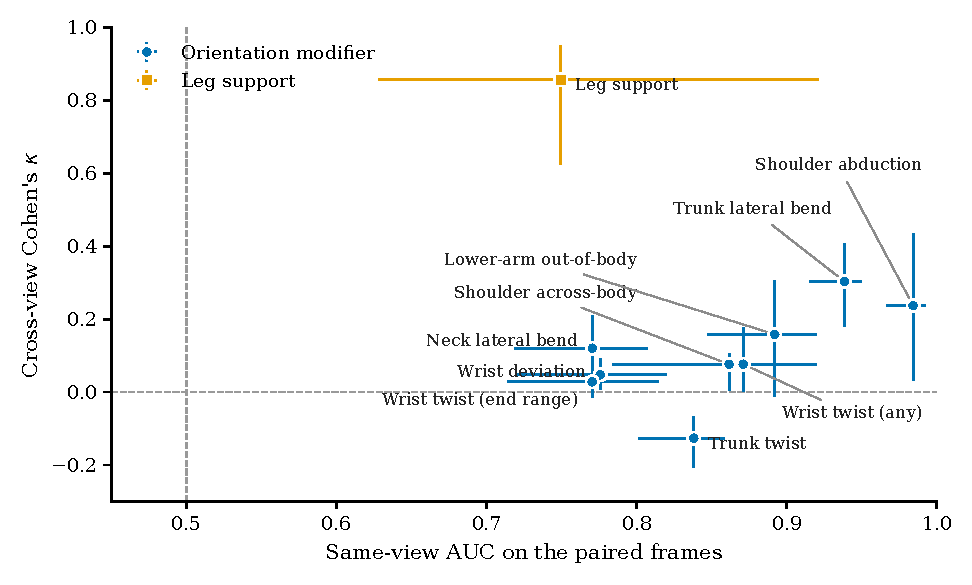
\includegraphics[width=\linewidth]{fig_paired.pdf}
\caption{Same-view AUC against cross-view Cohen's $\kappa$ for each modifier on the
\nXviewFrames\ frame pairs, with 95\% bootstrap intervals over the \nXviewSessions\ clip
pairs. Dashed lines mark chance on each axis. Upper-arm and trunk support are too rare on
the paired frames to plot.}
\label{fig:paired}
\end{figure}

\subsection{Against motion capture, out-of-plane predictions agree less between cameras than in-plane predictions}
\label{sec:andyresults}

Scored against the motion-capture labels, the single-camera predictions show how well one
camera recovers each posture. The better camera, the one with the higher AUC on a label, reaches
\andyAucTrunkTwist\ on trunk twist, the lowest of the \andyNLabels\ labels, and
\andyAucTrunkLateral\ to \andyAucTrunkFlexion\ on the other five (Table~\ref{tab:external}).
Camera 1, the other camera, reaches only \andyAucOneTrunkTwist\ on trunk twist, so how
well one camera recovers trunk twist depends on which camera it is. Of the
\andySweepN\ thresholds of the sweep, the highest leaves trunk twist and trunk lateral bend
too few positive frames in the training data of some fold, so both are scored at the other
\andySensEstTrunkTwist. At those thresholds, the trunk-twist AUC of the camera that is better at each threshold
ranges from
\andySensAucLoTrunkTwist\ to \andySensAucHiTrunkTwist. That AUC reaches \andyAucUsable, the lower
bound of acceptable discrimination \citep{hosmer2013logistic}, at only
\andySensRecovTrunkTwist\ of them, whereas trunk lateral bend reaches it at
\andySensRecovTrunkLateral\ and shoulder abduction at all \andySensEstArmAbd. The threshold
therefore decides whether one camera recovers trunk twist acceptably, whereas the other
two out-of-plane labels reach that bound at more than half of the thresholds. Each camera's
trunk-twist predictions agree with the motion-capture labels at
$\kappa=\andyFidKappaOneTrunkTwist$ and $\kappa=\andyFidKappaTwoTrunkTwist$, slight to fair
agreement, whereas its trunk-flexion predictions agree at
$\kappa=\andyFidKappaOneTrunkFlexion$ and $\kappa=\andyFidKappaTwoTrunkFlexion$, almost
perfect agreement.

Between the two cameras, the predictions agree at a mean $\kappa$ of \andyAdjOutOfPlane\
for the three out-of-plane labels, compared with \andyAdjInPlane\ for the three in-plane
labels, a difference of \andyGapMean\ (95\% CI [\andyGapMeanCiLo,\,\andyGapMeanCiHi]).
The out-of-plane label that agrees best, shoulder abduction at \andyAdjMaxOutOfPlane,
stays below the in-plane label that agrees worst, arm elevation at \andyAdjMinInPlane, by
\andyGapMin\ (95\% CI [\andyGapMinCiLo,\,\andyGapMinCiHi]; Table~\ref{tab:external}). The
mean $\kappa$ of the out-of-plane labels stays below that of the in-plane labels at every
threshold of the sweep at which all \andyNLabels\ labels can be scored.

\begin{table}[t]
\centering
\caption{Single-camera prediction of the AnDy labels from estimated 2-D pose, scored
against labels thresholded from Xsens motion capture. AUC is that of the camera that scores
higher. Agreement with the motion-capture labels is Cohen's $\kappa$ for camera 1 and camera
2. Cross-view $\kappa$ compares the two cameras' predictions for the same moment. Intervals
are 95\% bootstrap intervals over the \andyParticipants\ participants.}
\label{tab:external}
\small
\begin{tabular}{llccc}
\toprule
Label & Plane & AUC [95\% CI] & $\kappa$ with motion capture & Cross-view $\kappa$ [95\% CI] \\
\midrule
Trunk flexion & in-plane & \andyAucTrunkFlexion\ [\andyAucCiLoTrunkFlexion, \andyAucCiHiTrunkFlexion] & \andyFidKappaOneTrunkFlexion, \andyFidKappaTwoTrunkFlexion & \andyXviewKappaTrunkFlexion\ [\andyXviewKappaCiLoTrunkFlexion, \andyXviewKappaCiHiTrunkFlexion] \\
Neck flexion & in-plane & \andyAucNeckFlexion\ [\andyAucCiLoNeckFlexion, \andyAucCiHiNeckFlexion] & \andyFidKappaOneNeckFlexion, \andyFidKappaTwoNeckFlexion & \andyXviewKappaNeckFlexion\ [\andyXviewKappaCiLoNeckFlexion, \andyXviewKappaCiHiNeckFlexion] \\
Arm elevation & in-plane & \andyAucArmElev\ [\andyAucCiLoArmElev, \andyAucCiHiArmElev] & \andyFidKappaOneArmElev, \andyFidKappaTwoArmElev & \andyXviewKappaArmElev\ [\andyXviewKappaCiLoArmElev, \andyXviewKappaCiHiArmElev] \\
Shoulder abduction & out-of-plane & \andyAucArmAbd\ [\andyAucCiLoArmAbd, \andyAucCiHiArmAbd] & \andyFidKappaOneArmAbd, \andyFidKappaTwoArmAbd & \andyXviewKappaArmAbd\ [\andyXviewKappaCiLoArmAbd, \andyXviewKappaCiHiArmAbd] \\
Trunk lateral bend & out-of-plane & \andyAucTrunkLateral\ [\andyAucCiLoTrunkLateral, \andyAucCiHiTrunkLateral] & \andyFidKappaOneTrunkLateral, \andyFidKappaTwoTrunkLateral & \andyXviewKappaTrunkLateral\ [\andyXviewKappaCiLoTrunkLateral, \andyXviewKappaCiHiTrunkLateral] \\
Trunk twist & out-of-plane & \andyAucTrunkTwist\ [\andyAucCiLoTrunkTwist, \andyAucCiHiTrunkTwist] & \andyFidKappaOneTrunkTwist, \andyFidKappaTwoTrunkTwist & \andyXviewKappaTrunkTwist\ [\andyXviewKappaCiLoTrunkTwist, \andyXviewKappaCiHiTrunkTwist] \\
\bottomrule
\end{tabular}
\end{table}

\section{Discussion}
\label{sec:discussion}

\subsection{What a same-view AUC measures}
\label{sec:meaning}

Because the predictor matches each view's trunk-twist labels while the two views'
trunk-twist labels for the same moment agree below chance, the trunk-twist label depends on
the view for which it was set or on how that view was labeled. The trunk-twist same-view
AUC therefore records how well a predictor matches a view's trunk-twist label rather than
how well it recovers the trunk's rotation. An AUC that stays stable across camera angles does not separate matching
from recovery either, because a predictor scored against each view's own labels matches
each view's labels equally well whether or not the views agree. \citet{agostinelli2024validation} scored a pipeline against an assessment that ergonomists
made from the footage that the pipeline analyzed. A validation against an assessment made
from one view's footage cannot separate matching from recovery either, because the
assessment is itself a label of that view.

A reference that does not change with the view does separate them, as AnDy's motion-capture labels show by distinguishing trunk flexion, which one camera recovers almost
perfectly, from trunk twist, which it recovers at most fairly. No labeler set the AnDy
labels, so how labels were set cannot explain why the out-of-plane predictions agree less
between the two cameras than the in-plane predictions do. A multi-camera 3-D reconstruction
also recovered trunk twist, trunk lateral bend and shoulder abduction less accurately than
flexion \citep{vancrombrugge2022jointangles}. AnDy cannot show what makes the \datasetName's
labels disagree, however, because the two cameras' predictors are trained on one shared set of
motion-capture labels, whereas the two views of the \datasetName\ carry labels set separately.

The results of Section~\ref{sec:crossview} extend the observer disagreement that
\citet{schwartz2019reba} found on REBA to labels set from footage, which disagree between
two simultaneous views of one worker. The two views disagree most on trunk twist, which a
review of observational methods found seemed harder to observe correctly than the other
postures that it reviewed \citep{takala2010observational}. A pipeline trained to
match labels set from footage can therefore learn the labels' dependence on the view. Where the camera causes that
dependence, the pipeline's output changes with camera placement, which an instrument meant
to compare risk across workstations cannot allow. Validating such a pipeline therefore
needs labels that a second simultaneous view reproduces, or a reference that does not
change with the view. By that requirement, the \datasetName\ could validate only leg
support, and only on the pooled paired frames, because only leg support's labels agree
between the two views of a frame pair. Even against the labels of the view that the predictor sees, where the views'
disagreement plays no part, a score composed from the predicted modifiers agrees with the
labeled score only moderately. The points that the predicted modifiers add to or remove
from a frame's RULA score (\ref{app:rula}) agree with those of the labeled modifiers at a
linear-weighted $\kappa$ of \adjKappaTotal, a $\kappa$ that weights each disagreement by
its size.

\subsection{Limitations}
\label{sec:limits}

The comparison of the two views' labels is limited by its sample, by the timing of its frame pairs and by the dataset's record
of the labeling. Every paired frame comes from one of \nXviewWorkers\ workers at one plant,
so intervals that resample clip pairs treat clips of one worker as independent draws and
are narrower than intervals over workers would be. The near-simultaneous clips extend the
prevalence comparison to \nTakePairWorkers\ workers at \nTakePairFactories\ plants, but
they cannot give $\kappa$, which needs frames paired in time. The frame pairs' simultaneity
is inferred from start stamps that read a whole minute, because the dataset keeps no
synchronization record. The dataset also does not record whether one labeler handled both
views of a clip pair or whether labelers were assigned by camera, so a difference between
labelers could appear as a difference between views. The data guide does not say whether
the automatic suggestions were computed for each view or how often labelers kept them
unchanged, so suggestions computed from one view could carry that view into the labels.
Cross-view $\kappa$ therefore measures the combined effect of the view, the automatic
suggestion, the labeler and the inspector, not the view alone. The dataset's record also does not say which view's trunk-twist labels
are wrong, and neither can the prevalence gap, because the gap's direction differs between
workers.

The AnDy comparison and the same-view AUCs have limits of their own. On AnDy, both
cameras' predictors are trained on one shared set of motion-capture labels, which makes
their predictions agree more than labels set separately for each view would, so an AnDy
label's $\kappa$ overstates the agreement that separately set labels would reach. The posture bins alone reach an AUC of
\ablBinsUpperarmAbduct\ on shoulder abduction, so the abduction label may follow the
posture bin that the labeler set in the same frame rather than the arm angle that the skeleton shows, and
only a dataset that labels the bins and the modifiers independently could tell the two
sources apart. The same-view AUCs rest on \nSubjects\ workers at \nFactories\ plants, and
the dataset does not vary filming conditions such as illuminance within a worker, so the
AUCs may not hold under other conditions. The data guide notes that the camera angle that the dataset records for a clip was not
always the camera's actual facing direction, so the
per-angle AUCs of Section~\ref{sec:sameview} may mix directions. The dataset records neither the sex nor the
gender of its workers, so whether the results differ between the sexes or between genders is untested.

\section{Conclusions}
\label{sec:conclusions}

A predictor of RULA and REBA posture modifiers that is scored against labels set for the
view that it sees shows how well a skeleton recovers the posture only if the labels
describe the posture rather than the view. On factory video whose labels were set for each
camera's view, we scored a keypoint predictor against each view's labels and compared the
labels that two simultaneous views carry for one moment. On the frames that both views recorded, the annotated 2-D skeleton predicts each view's
orientation labels, whereas the two views' labels of every
orientation modifier agree at most fairly and those of trunk twist below chance. On a
second dataset labeled from motion capture, single-camera predictions of out-of-plane
labels agree less between two cameras than those of flexion and arm elevation. A high
same-view AUC therefore does not show how well the skeleton recovers the posture, so a
pipeline validated that way can report risk scores that change with where the camera
stands.

\section*{CRediT authorship contribution statement}
S.K. designed and conducted the research, performed the data analysis, and wrote the
manuscript.

\textbf{Sungwoo Kang:} Conceptualization, Methodology, Investigation, Formal analysis,
Writing -- original draft, Writing -- review and editing.

\section*{Funding}
This work received no funding.

\section*{Declaration of competing interest}
The author declares no known competing financial interests or personal relationships that
could have appeared to influence the work reported in this paper.

\section*{Declaration of generative AI and AI-assisted technologies in the manuscript
preparation process}
During the preparation of this work, the author used Claude (Anthropic) to assist with
code implementation as well as to improve the readability and language of the manuscript.
After using this tool, the author reviewed and edited the content as needed and takes full
responsibility for the content of the publication.

\section*{Data availability}
\label{sec:availability}
The study uses the \datasetName\ \citep{aihubmsk}, built under a project of the National
Information Society Agency (NIA) of the Republic of Korea and distributed through the AI
Hub portal. The author did not build the dataset and may not redistribute its images or
labels. AI Hub distributes it as a public dataset, although access is by
application. The portal's self-service application form accepts domestic applicants only,
whereas AI Hub's usage policy opens a separate route for applicants outside Korea by
agreement with NIA and the institution that built the dataset. The analysis code, the
result files and the frames' AI Hub file identifiers, which carry the worker and plant
keys, are available at \url{https://github.com/hpicsk/ergo-modifiers}. Re-running the analysis requires the dataset from AI Hub and AnDy, which its authors
distribute on Zenodo (\url{https://zenodo.org/record/3254403}). The result files carry every reported estimate
and interval, and the value from each of the \nSeeds\ splits behind every mean over the
splits. The folds are rebuilt from the worker and plant keys.

\appendix

\section{RULA input coverage and the composed modifier adjustment}
\label{app:rula}
\setcounter{table}{0}

RULA adds or removes points for the modifiers through terms that it calls Adjust terms.
The delivered modifiers supply each of RULA's $\rulaAdjustPlus$ and $\rulaAdjustMinus$
Adjust terms, except the two that the dropped modifiers of Section~\ref{sec:data} carry,
whereas no label records force or load or muscle use. The base posture band of each segment cannot be computed from the delivered labels,
because the bins' classes are not RULA's bands. The trunk bin is coarser than RULA's trunk
band. Rather than RULA's lower-arm band, the lower-arm bin holds
the three classes of the upper-limb code of the Ovako Working Posture Analysing System
(OWAS, \citealp{karhu1977owas}), an observational method. That code records whether both
arms are below shoulder level, one is at or above it, or both are. RULA's grand score, which
needs every input, therefore cannot be computed from the dataset (Table~\ref{tab:coverage}),
so this paper reports no grand score.

\begin{table}[!ht]
\centering
\caption{RULA input coverage by the delivered labels. A label is degenerate where it is
marked in almost every frame or in almost none. An input is degraded where the delivered
label measures something other than what the input needs, or where the label is
degenerate. An input is partial where its label
selects a column of RULA's look-up tables instead of adding points, and missing where no
label records it.}
\label{tab:coverage}
\small
\begin{tabular}{lll}
\toprule
RULA input & Delivered field & Status \\
\midrule
Trunk posture & trunk bin (coarser than RULA's band) $+$ bend/twist/support & degraded \\
Neck posture & neck bin $+$ lateral bend (twist degenerate) & degraded \\
Upper-arm posture & upper-arm bin $+$ abduction/support (elevation degenerate) & degraded \\
Lower-arm posture & (bin = OWAS upper-limb code) out-of-body/across-body$^\ddagger$ & degraded \\
Legs & leg support (the leg bin feeds no RULA input) & partial \\
Wrist posture & (no wrist bin) wrist deviation only & degraded \\
Wrist twist & wrist twist, any and end range & partial \\
Force / load & --- & missing \\
Muscle use / repetition & --- & missing \\
\bottomrule
\end{tabular}

\smallskip
{\footnotesize\raggedright $^\ddagger$The dataset records the across-body modifier with the
upper arm.\par}
\end{table}

The per-modifier predictions of Section~\ref{met:predictor} can be composed into RULA's
modifier adjustment, the sum of the Adjust terms, with each term's weight from
\citet{mcatamney1993rula}, which shows how the per-modifier AUCs carry into a score. Wrist
twist and leg support select a column of RULA's look-up tables rather than add a term, and
RULA counts trunk support inside the trunk's posture band rather than as an Adjust term,
so the two wrist-twist modifiers, leg support and trunk support stay out of the
adjustment.
Shoulder across-body and lower-arm out-of-body share the single $\rulaAdjustPlus$ that
RULA gives an arm working across the body or out to the side, so that term is
$\rulaAdjustPlus$ when either modifier is predicted. The base band is held fixed, which
cancels it from any comparison of prediction with label. The predicted adjustment agrees
with the labeled adjustment at linear-weighted $\kappa=\adjKappaTotal$, a $\kappa$ that
weights each disagreement by its size in points, and misses it by \adjMaeTotal\ points on
average (Table~\ref{tab:composition}). The predicted adjustment matches the labeled one
exactly on $\adjExactTotalPct\%$ of the frames. Upper-arm support
supplies the only Adjust term for contact with a surface, which agrees at
$\kappa=\adjKappaContact$. Upper-arm support
is mis-predicted in only $\adjContactSharePct\%$ of the frames whose adjustment is
mis-predicted, so nearly all of the adjustment's errors come from the orientation
modifiers. The orientation subtotal, the part of the adjustment that the orientation
modifiers supply, agrees at $\kappa=\adjKappaOrient$ at the threshold of \adjThreshold\ and at no higher $\kappa$ at any threshold from \adjThresholdLo\ to \adjThresholdHi.

\begin{table}[!ht]
\centering
\caption{Agreement of the predicted RULA modifier adjustment with the labeled adjustment,
base posture band held fixed, mean over the \nSeeds\ splits. Weighted $\kappa$
is linear, and the mean absolute error (MAE) is in adjustment points.}
\label{tab:composition}
\small
\begin{tabular}{lrr}
\toprule
Adjustment component & Weighted $\kappa$ & MAE (points) \\
\midrule
Total ($\adjGtMin$ to $\adjGtMax$) & \adjKappaTotal & \adjMaeTotal \\
Orientation subtotal & \adjKappaOrient & \adjMaeOrient \\
Contact term (upper-arm support) & \adjKappaContact & \adjMaeContact \\
\bottomrule
\end{tabular}
\end{table}

\clearpage
\section{Further checks of the keypoint predictor}
\label{app:checks}
\setcounter{table}{0}

Positive controls test whether the predictor's low AUC on upper-arm and trunk support comes
from the predictor rather than from the skeleton. The controls are a raised upper arm, a
bent trunk and bent legs, \ctrlNPairs\ postures that the posture bins record and that joint
positions show directly. Each is predicted under the protocol of
Section~\ref{met:predictor} with one split of the workers. The controls reach AUC \ctrlAucMin\ to
\ctrlAucMax. In every fold, the raised upper arm and the bent trunk reach an AUC at least
\ctrlMarginMin\ higher than the support modifier of the same body segment, so the
predictor learns the posture of the segments whose support it cannot predict. Bent legs,
however, reach a higher AUC than leg support in only \ctrlLegsFoldsWon\ of the \nFolds\
folds, because leg support itself goes with bent legs, so the leg control cannot show that
contrast.

A deployed pipeline takes its joints from a pose estimator rather than from annotation, so
we test whether the AUCs hold with estimated joints. Keypoint R-CNN, with the COCO
parameters of Section~\ref{met:andy}, estimates the pose in
\nCropsEst\ worker crops, the image regions inside the workers' bounding boxes. AI\,Hub
delivers the dataset in two parts, a training part and a validation part. The crops are
the whole validation part and, to bound the time spent decoding images, the first
\nCropsTrainCap\ crops of the training part in the order that its archive stores them.
On these crops, the estimator's percentage of correct keypoints, the share of joints that
it places within a tenth of the diagonal of the annotated joints' bounding box, is
$\posePckb\%$. It finds no worker in $\poseMissedPct\%$ of
the crops, whose joints are then all marked absent. Two predictors under the protocol of
Section~\ref{met:predictor} use the \nJointsEst\ body joints that the estimator and the
annotation share (the nose, shoulders, elbows, wrists, hips, knees and ankles). One takes
the annotated positions and the other the estimated positions
(Table~\ref{tab:estimatedpose}).
Replacing the annotated joints with estimated joints lowers no orientation modifier's AUC
by more than \poseMaxOrientDropAuc, and it changes the composed adjustment's $\kappa$ from
\adjKappaGtThirteen\ to \adjKappaEstThirteen. Both values are computed on the crops and
the \nJointsEst\ shared joints, whereas the \adjKappaTotal\ of \ref{app:rula} uses all
\nKeypoints\ keypoints on every frame.

\begin{table}[!ht]
\centering
\caption{Same-view AUC on the \nJointsEst\ body joints that Keypoint R-CNN shares with the
annotation, from the annotated joints and from the estimated joints, mean over the
\nSeeds\ splits. $\Delta$ is the annotated AUC minus the estimated AUC before
rounding.}
\label{tab:estimatedpose}
\small
\begin{tabular}{lrrr}
\toprule
Modifier & Annotated & Estimated & $\Delta$ \\
\midrule
Shoulder abduction & \aucGtUpperarmAbduct & \aucEsUpperarmAbduct & \dropUpperarmAbduct \\
Trunk lateral bend & \aucGtTrunkBend & \aucEsTrunkBend & \dropTrunkBend \\
Shoulder across-body & \aucGtUpperarmAcross & \aucEsUpperarmAcross & \dropUpperarmAcross \\
Trunk twist & \aucGtTrunkTwist & \aucEsTrunkTwist & \dropTrunkTwist \\
Lower-arm out-of-body & \aucGtLowerarmOut & \aucEsLowerarmOut & \dropLowerarmOut \\
Neck lateral bend & \aucGtNeckBend & \aucEsNeckBend & \dropNeckBend \\
Wrist deviation$^\dagger$ & \aucGtWristBend & \aucEsWristBend & \dropWristBend \\
Wrist twist (any)$^\dagger$ & \aucGtWristTwistAny & \aucEsWristTwistAny & \dropWristTwistAny \\
Wrist twist (end range)$^\dagger$ & \aucGtWristTwistEnd & \aucEsWristTwistEnd & \dropWristTwistEnd \\
Leg support & \aucGtLegsSupport & \aucEsLegsSupport & \dropLegsSupport \\
Upper-arm support & \aucGtUpperarmSupport & \aucEsUpperarmSupport & \dropUpperarmSupport \\
Trunk support$^\ddagger$ & \aucGtTrunkSupport & \aucEsTrunkSupport & \dropTrunkSupport \\
\bottomrule
\end{tabular}

\smallskip
{\footnotesize\raggedright $^\dagger$The shared joints include no hand keypoint.
$^\ddagger$Trunk support has almost no positives in the crops.\par}
\end{table}

\begin{table}[!ht]
\centering
\caption{Same-view AUC with workers held out of training (Table~\ref{tab:map}) and with
plants held out of training, mean over \nSeeds\ runs. With plants held out, the folds are
the plants, so the runs differ only in the random seed of training. $\Delta$ is the
worker-held-out AUC minus the plant-held-out AUC before rounding.}
\label{tab:unseenplant}
\small
\begin{tabular}{lrrr}
\toprule
Modifier & Worker held out & Plant held out & $\Delta$ \\
\midrule
Shoulder abduction & \aucUpperarmAbduct & \aucSiteUpperarmAbduct & \dropSiteUpperarmAbduct \\
Trunk lateral bend & \aucTrunkBend & \aucSiteTrunkBend & \dropSiteTrunkBend \\
Shoulder across-body & \aucUpperarmAcross & \aucSiteUpperarmAcross & \dropSiteUpperarmAcross \\
Trunk twist & \aucTrunkTwist & \aucSiteTrunkTwist & \dropSiteTrunkTwist \\
Lower-arm out-of-body & \aucLowerarmOut & \aucSiteLowerarmOut & \dropSiteLowerarmOut \\
Neck lateral bend & \aucNeckBend & \aucSiteNeckBend & \dropSiteNeckBend \\
Wrist deviation & \aucWristBend & \aucSiteWristBend & \dropSiteWristBend \\
Wrist twist (any) & \aucWristTwistAny & \aucSiteWristTwistAny & \dropSiteWristTwistAny \\
Wrist twist (end range) & \aucWristTwistEnd & \aucSiteWristTwistEnd & \dropSiteWristTwistEnd \\
Leg support & \aucLegsSupport & \aucSiteLegsSupport & \dropSiteLegsSupport \\
Upper-arm support & \aucUpperarmSupport & \aucSiteUpperarmSupport & \dropSiteUpperarmSupport \\
Trunk support$^\ddagger$ & \aucTrunkSupport & \aucSiteTrunkSupport & \dropSiteTrunkSupport \\
\bottomrule
\end{tabular}

\smallskip
{\footnotesize\raggedright $^\ddagger$Not a valid estimate, because almost all trunk-support
positives lie in one plant.\par}
\end{table}

\begin{table}[!ht]
\centering
\caption{Same-view AUC on the \nXviewFrames\ frame pairs in four forms. The first view of a
pair is the view from the camera angle with the lower number. The first column pools the first views of all pairs, and the second column their second
views. The third and fourth columns score both views together, as Table~\ref{tab:crossview}
does. The third comes from a predictor trained without the plant of the paired frames,
and the fourth averages the AUC within each clip pair over the clip pairs with frame
weights.}
\label{tab:pairedchecks}
\small
\begin{tabular}{lrrrr}
\toprule
Modifier & First view & Second view & Plant held out & Within clip pairs \\
\midrule
Shoulder abduction & \pairAucFirstUpperarmAbduct & \pairAucSecondUpperarmAbduct & \plantPairAucUpperarmAbduct & \withinPairAucUpperarmAbduct \\
Trunk lateral bend & \pairAucFirstTrunkBend & \pairAucSecondTrunkBend & \plantPairAucTrunkBend & \withinPairAucTrunkBend \\
Shoulder across-body & \pairAucFirstUpperarmAcross & \pairAucSecondUpperarmAcross & \plantPairAucUpperarmAcross & \withinPairAucUpperarmAcross \\
Trunk twist & \pairAucFirstTrunkTwist & \pairAucSecondTrunkTwist & \plantPairAucTrunkTwist & \withinPairAucTrunkTwist \\
Lower-arm out-of-body & \pairAucFirstLowerarmOut & \pairAucSecondLowerarmOut & \plantPairAucLowerarmOut & \withinPairAucLowerarmOut \\
Wrist deviation & \pairAucFirstWristBend & \pairAucSecondWristBend & \plantPairAucWristBend & \withinPairAucWristBend \\
Wrist twist (any) & \pairAucFirstWristTwistAny & \pairAucSecondWristTwistAny & \plantPairAucWristTwistAny & \withinPairAucWristTwistAny \\
Wrist twist (end range) & \pairAucFirstWristTwistEnd & \pairAucSecondWristTwistEnd & \plantPairAucWristTwistEnd & \withinPairAucWristTwistEnd \\
Neck lateral bend & \pairAucFirstNeckBend & \pairAucSecondNeckBend & \plantPairAucNeckBend & \withinPairAucNeckBend \\
Leg support & \pairAucFirstLegsSupport & \pairAucSecondLegsSupport & \plantPairAucLegsSupport & \withinPairAucLegsSupport \\
\bottomrule
\end{tabular}
\end{table}

\clearpage
\section{Predictor settings and AnDy synchronization}
\label{app:settings}

The LightGBM ensemble of Section~\ref{met:predictor} has \lgbmTrees\ trees. Each tree has
at most \lgbmLeaves\ leaves (end nodes), with at least \lgbmMinLeaf\ frames per leaf. A
learning rate of \lgbmRate\ scales each tree's contribution, and each tree may use a share
of \lgbmFeatureFraction\ of the input variables, the feature fraction. Each
predictor gives every positive training frame a weight equal to the ratio of negative to
positive training frames, so that a rare modifier is not ignored in training.

For each pair of the three recordings of an AnDy trial (Section~\ref{met:andy}), we
cross-correlate over time the vertical positions of the body centroid, the head and the
forearms, which the nose and the wrists stand for in the videos, and take the time offset
at the peak correlation. The offset between the cameras must equal the difference of the two cameras'
offsets from the motion capture, and the residual of that equality checks each trial. On
\andySyncValTrials\ trials whose offsets we also checked by eye against the videos, the
median residual is \andySyncResidMed\,s. A trial enters the comparisons with the
motion-capture labels when the peak correlation of each of the three pairs reaches
\andySyncCorrMin\ and the residual is at most \andySyncResidMax\,s, values that we chose
from the trials checked by eye. A trial enters the comparison between the cameras when the
peak correlation of the two cameras reaches \andySyncCorrMin.

\bibliographystyle{elsarticle-harv}
\bibliography{references}

\end{document}
